 
\chapter{Applications of the discrete Fourier transform}
\label{chap-applications-tfd} 
 
 
 
We therefore saw, in the previous chapter, that we have an efficient algorithm, the FFT algorithm, to calculate the discrete Fourier transform. From then on, all applications using Fourier theory from near or far will be able to benefit from this algorithmic \guill{find}. But this phenomenon goes even further, since many other problems, however far removed from harmonic analysis, will be solved quickly thanks to the FFT algorithm. We will thus see that we can quickly calculate products of large integers, or even approach the solution of the Poisson equation, which may seem somewhat disconnected from the concerns we had until then!
 
% ------------------------------------------------- -----
% ------------------------------------------------- -----
% ------------------------------------------------- -----
% section - Link with the Fourier transform on $ \RR $                            
% ------------------------------------------------- -----
% ------------------------------------------------- -----
% ------------------------------------------------- -----
\section{Link with the Fourier transform on $ \RR $}
% \addcontentsline{toc}{section}{Link with the Fourier transform on $ \RR $}
\label{sect1-link-trans-fourier-R} 
 
This chapter is above all useful to better understand intuitively the discrete Fourier transform, thanks to many analogies with the continuous Fourier transform. It is not there to give the DFT a numerical nature, because it is above all necessary to conceive the discrete transform as an algebraic transformation, with an exact reconstruction formula (the inverse discrete Fourier transform). However, it is true that the FFT algorithm is often used to calculate Fourier coefficients in an approximate way, even if we will quickly see that the corresponding quadrature formula is not very precise.
% ------------------------------------------------- -----
% ------------------------------------------------- -----
% sub-section - Continuous Fourier transform                            
% ------------------------------------------------- -----
% ------------------------------------------------- -----
\subsection{Continuous Fourier transform}
\label{sect2-transforme-fourier-continue} 
 
 
\index{Fourier transform!on $ \RR $} We have just defined, in a way that we could qualify as abstract, the discrete Fourier transform. We can therefore naturally wonder if the latter has any relation to the usual Fourier transform on $ \RR $. The latter, for a function $ f \in L^1 (\RR) $ is defined by the equation
\begin{equation}
\label{eq-transforme-fourier-R}
\forall \xi \in \RR, \quad \wh{f} (\xi) \eqdef \int_{\minf}^{\pinf}{f(t) e^{- \imath \xi t} \d t}.
\end{equation}
This functional transformation has a very important meaning, particularly in the field of signal processing. If we consider that the function $ f $ represents a continuous signal which propagates in time, the Fourier transform makes it possible to pass from a temporal representation to a frequency representation. The quantity $ \wh{f} (\xi) $ intuitively represents how many variations there are at the frequency $ \xi $ in $ f $.
 
 
Moreover, we can extend by density the Fourier transform to functions $ f \in L^2 (\RR) $ of finite energy, i.e. such that $ \int_{\RR}{| f(x) |^2 \d x} <+ \infty $. Thus, the famous formula of \textit{Parseval}:
\begin{equation*}
\forall f \in L^2 (\RR), \quad \norm{\wh{f}}_{L^2} = 2 \pi \norm{f}_{L^2}
\end{equation*}
can be interpreted as a conservation of energy during the transition from the time domain to the frequency domain. For more details on the construction of the Fourier transform on $ \RR $, one can consult the book of \nompropre{Rudin} \cite{rudin}.
 
 
As for the Fourier transform on a finite group, we also have an inversion theorem, under somewhat restrictive assumptions.
 
\begin{prop}[Inversion formula]
\index{Inversion formula} When $ f \in L^2 $ and $ \wh{f} \in L^1 $, we have almost everywhere
\begin{equation}
\label{eq-formula-inversion-R}
f(x) = \frac{1}{2 \pi} \int_{\RR}{\wh{f} (\xi) e^{\imath x \xi} \d \xi}.
\end{equation}
\end{prop}
In fact, we could redo a character theory on the group $ (\RR, +) $ as it was done on finite abelian groups. Here is for example the determination of the characters of the real line:
 
\begin{prop}[Characters from $ \RR $]
\label{prop-characters-r}
\index{Character!of $ \RR $} \label{notation-52} We name the character of $ (\RR, +) $ the continuous morphisms of $ \RR $ in $ \Gamma \eqdef \enscond{z \in \CC}{| z | = 1} $. As usual, we denote by $ \wh{\RR} $ the group formed by the characters. For $ \gamma \in \RR $, either
\begin{equation*}
e_{\gamma}: \func{\RR}{\CC^*}{t}{e^{\imath \gamma t}}.
\end{equation*}
So we have $ \wh{\RR} = \{e_{\gamma} \}_{\gamma \in \RR} $ and the application $ \gamma \mapsto e_{\gamma} $ is an isomorphism between $ \RR $ and $ \wh{\RR} $.
\end{prop}
\begin{proof}
The $ e_{\gamma} $ are of course elements of $ \wh{\RR} $. Let $ \chi $ be a continuous morphism from $ \RR $ to $ \Gamma $. We will start by showing that $ \chi $ is a differentiable function. To do this, it suffices to integrate the homomorphism property in the neighborhood of $ 0 $:
\begin{equation*}
\int_0^h{\chi (s + t) \d t} = \chi (s) \int_0^h{\chi (t) \d t}.
\end{equation*}
As $ \chi (0) = 1 $, for $ h $ small enough, we have $ \int_0^h{\chi (t) \d t} \neq 0 $. We therefore have, for a certain $ h $,
\begin{equation*}
\chi (s) = \frac{\int_s^{h + s}{\chi (t) \d \d tt}}{\int_0^h{\chi (t) \d t}},
\end{equation*}
which clearly defines a continuously differentiable function. Note $ \lambda = \chi'(0) $. By factoring the rate of increase, we obtain
\begin{equation*}
\forall s \in \RR, \quad \chi'(s) = \lim_{t \rightarrow 0}{\frac{\chi (s + t) - \chi (t)}{h}} = \chi (s) \lim_{t \rightarrow 0}{\frac{\chi (t) - \chi (0)}{h}} = \lambda \chi (s).
\end{equation*}
Note that the only function $ f $ which checks $ f'= \lambda f $ and $ f(0) = 1 $ is $ s \mapsto e^{\lambda s} $. It only remains to show that $ \lambda \in \imath \RR $. Just use $ \chi (s) \ol{\chi (s)} = \chi (0) = $ 1. By differentiating this equality in 0, we find $ \lambda + \ol{\lambda} = 0 $.
\end{proof}
Thus, the inversion formula \eqref{eq-formula-inversion-R} is to be compared to the formula \eqref{prop-decomposition-serie-fourier}, on a finite group: we were in a way content to replace the sum finite by an integral. Similarly, we could analyze the decomposition of a function $ 2 \pi $ -periodic in Fourier series. This time, it would be to use the characters in the circle $ S^1 \eqdef \RR / 2 \pi \ZZ $, which are the functions
\begin{equation*}
\forall n \in \ZZ, \; \forall t \in \RR, \quad e_n (t) \eqdef e^{int}.
\end{equation*}
The decomposition formula of a periodic Fourier series function (under good assumptions, and specifying the direction of convergence) is once again an inversion formula, this time with a countable sum. For an introduction to Fourier series and integrals on a group, one can consult the book of \nompropre{Dym} and \nompropre{MacKean} \cite{dym}, chapter 4.
% ------------------------------------------------- -----
% ------------------------------------------------- -----
% sub-section - Approximate calculation of the Fourier transform on $ \RR $                            
% ------------------------------------------------- -----
% ------------------------------------------------- -----
\subsection{Approximate calculation of the Fourier transform on $ \RR $}
\label{sect2-calculus-trans-fourier-approach} 
 
 
\index{Calculus!approximate integrals} \index{Translation} Before embarking on approximate calculations of integrals, it is necessary to be aware that the discrete Fourier transform is not limited to such approximations. We can partly explain the \guill{intuitive} properties of the discrete Fourier transform by invoking approximations of the continuous Fourier transform. However, what makes the discrete Fourier transform work so well does not come from its ability to faithfully approach the continuous transform (it is even the opposite), but comes from the fact that it transposes the algebraic properties that we used for the real line (convolution, inversion, translation, ...) in the case of a finite and cyclic domain. It is therefore the algebraic properties of the DFT which make it a powerful tool in numerical analysis, and which make it possible to have simple and fast algorithms. In this paragraph, we will nevertheless explain the connections which connect, in terms of approximate calculations, the two transforms, discrete and continuous.
 
 
\index{Method!of rectangles} Of course, the correct method to approximate the continuous transform is to find the value of $ \wh{f} $ at certain points. Indeed, we know in practice the signal $ f $ only in the form of a sample $ \{f [n] \}_{n = 0}^{N-1} $, each value $ f [n ] $ being measured for a value of the parameter $ x $ equal to $ x_n \eqdef n \Delta $, for $ n = 0, \ldots, \, N-1 $. $ \Delta $ is the discretization step, that is to say the interval (of time if we consider a signal varying in time) between two measurements of the signal $ f $.
 
 
In the following, in order to simplify the explanations, it is assumed that $ N $ is an even integer. It is clear that given a sample of $ N $ values of the signal $ f $, it is futile to want to compute more than $ N $ independent values of the Fourier transform $ \wh{f} $. This intuitive remark will be confirmed by the following approximate calculation:
\begin{equation*}
\forall \xi \in \RR, \quad \wh{f} (\xi) \approx \Delta \sum_{n = 0}^{N-1}{f [n] e^{- \imath \xi x_n}}.
\end{equation*}
This approximation is obtained by using the method of the rectangles on the left to calculate in an approximate way the integral \eqref{eq-transforme-fourier-R}. For this approximation to have a meaning, it is of course necessary that outside the interval $ [0, \, N \Delta] $ the function $ f $ is otherwise zero, at least very rapidly decreasing.
 
 
We see then that by calculating the values of $ \wh{f} $ for values of the parameter $ \xi $ of the form $ \xi_k \eqdef \frac{2k \pi}{N \Delta} $ we obtain a writing particularly pleasant for the approximate calculation of $ \wh{f} (\xi_k) $:
\begin{equation}
\label{eq-approx-transforme-fourier-dft-1}
\wh{f} (\xi_k) \approx \Delta \sum_{n = 0}^{N-1}{f [n] e^{\frac{- 2 \imath \pi}{N} kn}} .
\end{equation}
As we mentioned before, it makes sense to only calculate $ N $ values of the Fourier transform, so we will apply the previous calculation to the points $ \xi_k $ for $ k $ variant in $ \{- N / 2 + 1, \ldots, \, N / 2 \} $. One might ask why we don't start at the index $ k = -N / 2 $, but we see that we get the same result for $ \xi_{- N / 2} $ and for $ \xi_{N / 2} $ (which conforms to our idea: no need to calculate more than $ N $ coefficients). By comparing the expression \eqref{eq-approx-transforme-fourier-dft-1} and the definition of the discrete Fourier transform \eqref{eq-defn-tfd}, we obtain
\begin{equation}
\label{eq-approx-transforme-fourier-dft}
\forall k \in \{0, \ldots, \, N-1 \}, \quad \wh{f} (\xi_k) \approx \Delta \wh{f}[k],
\end{equation}
where we have denoted $ \wh{f}[k] $ the \ordin{k}{ième} input of the discrete Fourier transform of the vector $ \{f [0], \ldots, \, f [N -1] \} \in \CC^N $ (as defined by the equation \eqref{eq-defn-tfd}).
 
 
However, there is a slight trick in the \eqref{eq-approx-transforme-fourier-dft} equation. Indeed, the index $ k $ varies in $ \{-N / 2 + 1, \ldots, \, N / 2 \} $, while the discrete transform vector $ \{\wh{f}[0 ], \ldots, \, \wh{f}[N-1] \} $ has its indices in $ \{0, \ldots, \, N-1 \} $. It is nevertheless easy to see that we did not make an error in writing the equality \eqref{eq-approx-transforme-fourier-dft}, since the discrete transform vector can be seen as a periodic function of period $ N $. We can therefore replace the negative frequencies $ \{- N / 2 + 1, \ldots, \, -1 \} $ by the frequencies $ \{N / 2 + 1, \ldots, \, N-1 \} $ : we get a vector whose indices vary between $ 0 $ and $ N-1 $.
 
 
Thus, the formula \eqref{eq-approx-transforme-fourier-dft} tells us that up to a factor $ \Delta $, the vector of the discrete Fourier transform $ \{\wh{f}[0], \ldots, \, \wh{f}[N-1] \} $ represents an approximation of the Fourier transform of the signal $ f $, but taken at very specific frequencies: the indices $ n $ between $ 0 $ and $ N / 2-1 $ correspond to the positive frequencies between $ 0 $ and $ f_c \eqdef \frac{\pi}{\Delta} $ (excluded), the indices $ n = N / 2 + 1, \ldots, \, N -1 $ correspond to the negative frequencies between $ -f_c $ (excluded) and $ 0 $ (excluded), while the index $ N / 2 $ corresponds to both the frequency $ f_c $ and $ -f_c $ (which is normal, since the transformed discrete signal is periodic with period $ N $). We must therefore pay attention to the following two points. \begin{rs}
\item The transformed vector $ \{\wh{f}[0], \ldots, \, \wh{f}[N-1] \} $ is considered as a periodic data of period $ N $ (it is the proper of the Fourier transform on an abelian group, in this case $ \ZZ/N \ZZ $). This is of course not the case with the function $ f: \RR \rightarrow \CC $ which has no reason to be periodic with period $ 2 f_c $.
\item Compared to the Fourier transform on $ \RR $ of the continuous signal $ f $, the frequencies are arranged in the order: negative frequencies, then positive frequencies.
\end{rs}
% ------------------------------------------------- -----
% ------------------------------------------------- -----
% sub-section - Addition of zeros                            
% ------------------------------------------------- -----
% ------------------------------------------------- -----
\subsection{Addition of zeros}
\label{sect2-addition-zeros} 
 
\index{Zero padding} There are two basic techniques for influencing how one can calculate, using the discrete transform, different values of the continuous transform. \begin{rs}
\item \index{Sampling} We can sample the signal with more or less precision. We have seen that the more precise the sampling is (that is to say the more points we take to represent the analyzed function), the wider the spectrum of the transform. Thus, if one wishes to cover a spectrum twice as large, it suffices to divide the interpolation interval by two. Of course, this also extends the time needed to do the math.
\item You can add zeros at the end of the vector. If we are satisfied with the spectrum on which we calculate the transform (more precisely the maximum and minimum frequencies that we can calculate), we may then want to calculate the transform with more precision, for example if we want to draw a curve to graphically represent the transform. In this case, the procedure is simple: it suffices to add zeros at the end of the vector, to add as many calculated intermediate frequencies.
\end{rs} By playing on these two parameters (interpolation precision and addition of zeros), we can calculate \guill{custom} discrete transforms, to have a certain fixed vector size (this can be used to create filters, see Section~\ref{sect1-filtering}), but also for the representation of the transform. The figure \figref{fig-calcul-approach-tf} shows the different results that can be obtained by adjusting both the number of sampling points and the addition of zeros. The functions represented are the modules of the DFT of the indicator function of $ [0.5, \, 1] $, sampled on $ [0, \, 1] $ at regular intervals. Each row uses the same number of sample points, but with more or less zeros added. \begin{figure}[ht]
    \begin{center}
    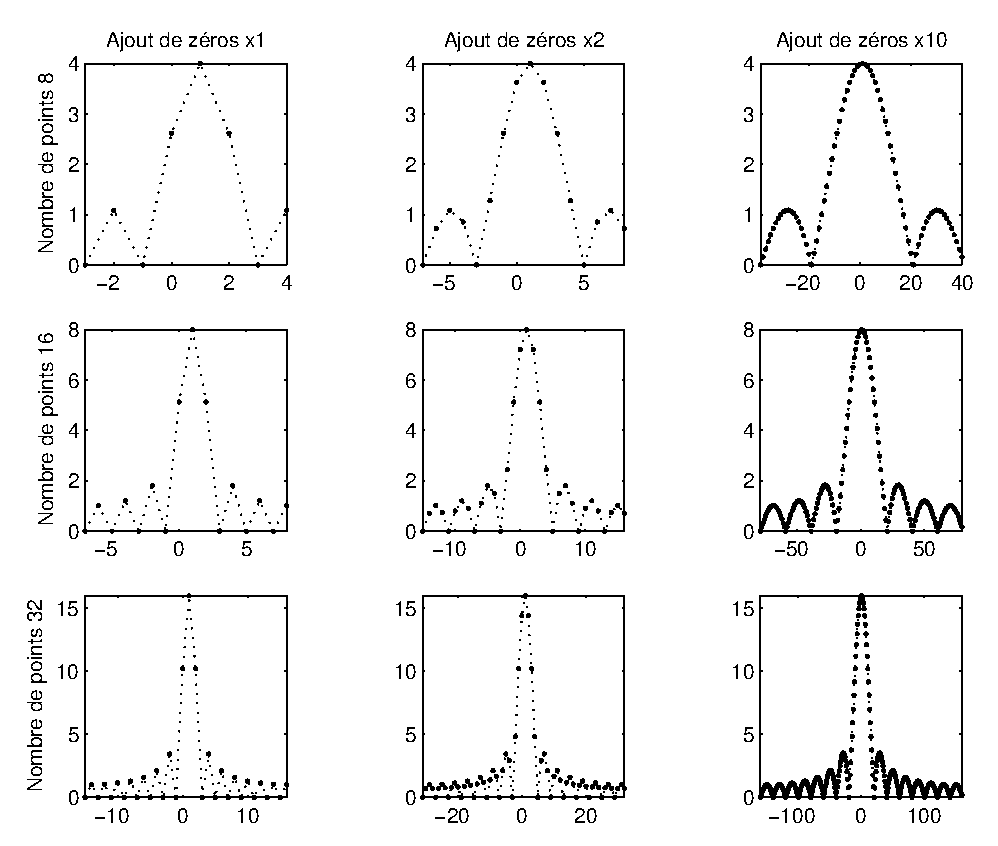
\includegraphics[scale=0.7]{images/calcul-approche-tf.eps}
    \end{center}
    \caption{Influence of sampling and adding zeros}
              \label{fig-calcul-approach-tf}
\end{figure}
The exercise \oldref{exo-creation-low-pass-filter} is instructive in this regard, since it reinvests all of this in order to create and test a low-pass filter.
% ------------------------------------------------- -----
% ------------------------------------------------- -----
% sub-section - Time / frequency duality                            
% ------------------------------------------------- -----
% ------------------------------------------------- -----
\subsection{Time / frequency duality}
\label{sect2-duality-time-frequency} 
 
 
\index{Uncertainty!principle} \index{Uncertainty} The approximate calculation we have just done allows us, via the use of the discrete Fourier transform, to calculate the value of the Fourier transform of a signal for certain frequencies only, precisely those of the form $ \frac{2 k \pi}{N \Delta} $ for $ k \in \{- N / 2 + 1, \ldots, \, N / 2 \} $. We therefore notice that the greater the precision with which the computation is carried out (that is to say the discretization step $ \Delta $ is small), the more the spectrum on which the transform is calculated is spread. This is not an isolated phenomenon, and results from a very strong duality between the starting function and its Fourier transform.
 
 
The following result clearly illustrates this duality between the temporal properties of a signal (that is to say the properties of a function $ f $) and its frequency properties (that is to say those of the transformed function $ \wh{f} $).
 
\begin{prop}
\label{prop-trans-fourier-support-compact}
\index{Support!compact} Let $ f $ be a function of $ L^2 (\RR) $. Then $ f $ and $ \wh{f} $ cannot simultaneously be compactly supported.
\end{prop}
The proof of this result is given in the exercise \oldref{exo-transforme-sup-comp}. This property has an immediate discrete analogue, which we can see by considering the discrete impulse $ \delta_0 $ (the vector which is worth 1 in 0, and which is zero everywhere else). Its discrete Fourier transform has a spectrum that covers the entire interval considered, since it is the exponential function $ t \mapsto e^{2 \imath \pi t} $ sampled at regular time intervals.
% ------------------------------------------------- -----
% ------------------------------------------------- -----
% ------------------------------------------------- -----
% section - Filtering                            
% ------------------------------------------------- -----
% ------------------------------------------------- -----
% ------------------------------------------------- -----
\section{Filtering}
% \addcontentsline{toc}{section}{Filtering}
\label{sect1-filtering} 
 
\index{Filter} The notion of filtering a sampled signal is easy to define, but is used in an intensive and varied manner. We will therefore not go around the question, however, it is interesting to link the technique of filtering with tools such as the FFT algorithm and linear convolution.
% ------------------------------------------------- -----
% ------------------------------------------------- -----
% sub-section - Linear filters                            
% ------------------------------------------------- -----
% ------------------------------------------------- -----
\subsection{Linear filters}
\label{sec2-linear-filters} 
 
 
\index{Filter!linear} \label{notation-53} Let us start by defining the filtering of a theoretical infinite signal, before looking at the practical computation on finite signals. The filtering of a signal $ f \in \CC^\ZZ $ consists in pairing (acyclically of course) this signal with another signal $ g \in \CC^\ZZ $ fixed in advance. We thus obtain a filter operator
\begin{equation*}
\Phi^g: \func{\CC^\ZZ}{\CC^\ZZ}{f}{f \star g}.
\end{equation*}
\index{Transfer!function} We say that $ g $ is the transfer function of the filter $ \Phi^g $.
 
 
\index{Impulse!response} One of the remarkable properties of linear filters is that they obtain the \textit{impulse response} (that is, how the system represented by the filter reacts to an impulse), which is calculated very simply:
\begin{equation*}
\Phi^g (\delta_0) = \delta_0 \star g = g,
\end{equation*}
where we noted $ \delta_0 $ the impulse in $ 0 $, that is to say the sequence which is worth $ 1 $ in $ 0 $, and which is zero everywhere else (we speak of \textit{discrete Dirac}). In other words, the filter transfer function is nothing more than the impulse response.
 
 
\index{Support} Once all these definitions have been exposed, we have to ask ourselves the question of the practical calculation of the filter. If we want to be able to calculate the convolution $ f \star g $ in a finite time, a natural assumption is to impose on the impulse response $ g $ to be finite (more precisely with finite support). It is a rather radical choice, but the interest is that it will allow us to apply a linear filter to finite signals in a very simple way. It will indeed suffice to use the acyclic convolution techniques already presented in Section~\ref{sect1-convolution-acyclic}. Let us briefly recall the procedure to follow. We suppose that the signal to be filtered is of the type: $ f = \{f [0], \ldots, \, f [N-1] \} $, and that the impulse response, it, is can be defined for negative indices, but is, in all cases, of finite size $ P $. We must: \begin{rs}
\item add enough zeros to the two vectors so that they reach the size of $ N + P-1 $.
\item move the negative index entries $ g $ to the end of the vector (this is customary for cyclic convolutions).
\item calculate the convolution \textit{cyclic} by FFT then inverse FFT.
\item extract the indices that interest us from the result and put them back in order (if we want to retrieve the entries with negative indices).
\end{rs}
 
 
One of the main characteristics of the convolution filters that we have just described is that they have a finite impulse response, in the sense that it becomes zero outside the support of $ g $. This is why we often name the convolution filters \textit{finite impulse response filters}, in English \textit{FIR} (for \textbf{F} inite \textbf{I} mpulse \textbf{R} esponse). We will see in Paragraph~\ref{sect2-application-trans-z-filters}, that we can easily build filters which do not have this property, but which can still be calculated in a finite time.
 
 
In most cases, the transfer function $ g $ has limited support in the neighborhood of $ 0 $ (that is, only inputs in the neighborhood of $ 0 $ are non-zero). A good example is the Gaussian filter, given by the equation
\begin{equation*}
\forall k \in \{- N / 2, \ldots, \, N / 2 \}, \quad g [k] = \frac{1}{M} \exp \left(- \frac{(2 k / N)^2}{2t} \right).
\end{equation*}
The parameter $ M $ is adjusted so that $ \norm{g}_1 \eqdef \sum_k{| g [k] |} = $ 1. The parameter $ t $ represents the variance of the Gaussian. The smaller $ t $, the more the Gaussian is \guill{picked}, so the more $ g $ tends towards the Dirac $ \delta_0 $ (and the filter $ \Phi^g $ tends towards the identity). On the contrary, the larger $ t $ becomes, the more the Gaussian is \guill{spread}, and the more the filter smooths the signal. We must pay attention to the fact that the indices of $ g $ have been taken from $ [- N / 2, \, N / 2] $, because we want to realize an acyclic filter. To perform a cyclic filter and / or calculate the filter by FFT, it is of course necessary to report the negative frequencies \textit{at the end} of the vector.
 
 
Figure \figref{fig-filter-smoothing} shows different Gaussian kernels (top). The left kernel has a variance $ t $ so low that it is equal to the Dirac. The bottom line shows the filtering of an irregular signal (shown on the left, since filtering by a Dirac has no effect). We see that the higher the variance, the more regular the filtered signal. This joins the classical theory of continuous convolution: when we filter by a kernel of class $ \Cc^\infty $ (for example a Gaussian), the function instantly becomes of class $ \Cc^\infty $, therefore extremely smooth!\begin{figure}[ht]
    \begin{center}
    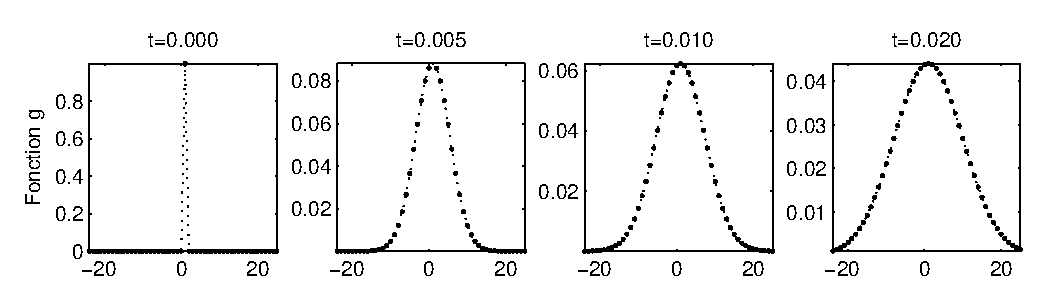
\includegraphics[scale=0.7]{images/filtre-lissage-1.eps}
    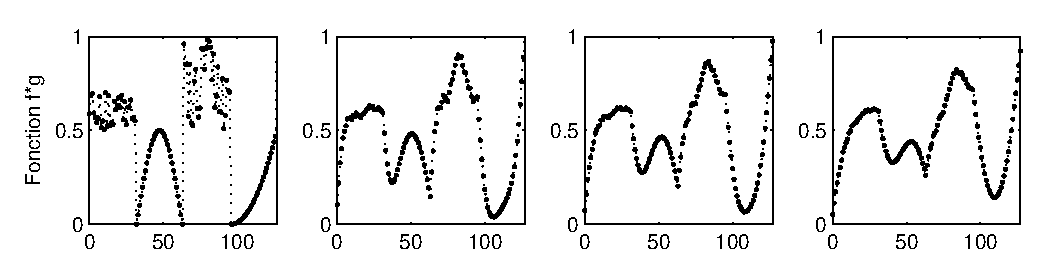
\includegraphics[scale=0.7]{images/filtre-lissage-2.eps}
    \end{center}
    \caption{Smoothing by a Gaussian}
              \label{fig-filter-smoothing}
\end{figure}
 
% ------------------------------------------------- -----
% ------------------------------------------------- -----
% sub-section - Types of responses and stability                            
% ------------------------------------------------- -----
% ------------------------------------------------- -----
\subsection{Response types and stability}
\label{sect2-responses-stability} 
 
 
We have therefore seen that the impulse response defines a filter. However, we can also characterize this filter by other types of responses, including: \begin{rs}
\item \index{Harmonic} \index{Frequency response} \textit{the frequency response}. It is simply the Fourier transform of the transfer function, i.e. $ \sum_{k \in \ZZ}{g [k] e^{\imath kx}} $, for $ x \in [- \pi, \, \pi] $. It is a $ 2 \pi $ -periodic function, since it is the Fourier series associated with the coefficients $ g [k] $. Since the impulse response $ g $ is finite, we can calculate it by discrete transform (FFT), by adding a lot of zeros at the end of $ g $ to have a very good precision (a quasi-continuous plot of the function, cf paragraph \ref{sect2-addition-zeros}). It represents how the filter operates in the frequency domain. Indeed, by using the convolution theorem \ref{prop-convol-tfd}, we see that the frequency response indicates by what quantity the filtering will multiply the amplitude of each harmonic (i.e. each component of the transformed vector) of the original signal.
\item \index{Step!Response} \textit{Step Response}. This is the vector obtained by filtering a step, that is to say the sequence which is zero for negative indices, and which is worth $ 1 $ for indices equal to or greater than $ 0 $. This response indicates how the filter will react to a discontinuity. For a normally constituted human mind, this is the answer that makes the most sense, since the human eye is above all trained to spot discontinuities. Thus, by observing the step response of a 2D filter, we will have indications on how the filter will transform the contours of the image (where there is a strong variation in intensity).
\end{rs} In a pragmatic way, the frequency response is calculated very simply by using the FFT algorithm (by taking care to add enough zeros to obtain sufficient precision, and by putting the negative frequencies back in their place) . For the step response, there are at least two ways to proceed. \begin{rs}
\item \index{Echelon} We can give a step at the input of the filter. For linear filtering, it suffices to give as input a constant vector equal to $ 1 $, the algorithm being supposed to add enough zeros to avoid circular convolution.
\item If we know the impulse response $ y_0 $ and we want to calculate the step response $ y_1 $, it suffices to notice that the step function is the discrete primitive (that is to say the partial sum), and therefore using the linearity of the filter, it will be the same for both responses. We thus obtain the simple formula
\begin{equation*}
\forall n \geq 0, \quad y_1 [n] = \sum_{k = \minf}^{n}{y_0 [k]}.
\end{equation*}
\end{rs} 
Figure \figref{fig-diff-types-responses} shows the three different response types for 3 different transfer functions. The first line represents a Gaussian, and we can see that the impulse response is also a Gaussian (which is logical, since the transform of a Gaussian is Gaussian, see the lemma \ref{lem-tf-gaussienne}). The other two lines show filters with a slower decay, and there are some oscillations in the frequency response. Note that filters are not causal, i.e. transfer functions are defined for negative indices. 

\begin{figure}[ht]
    \begin{center}
    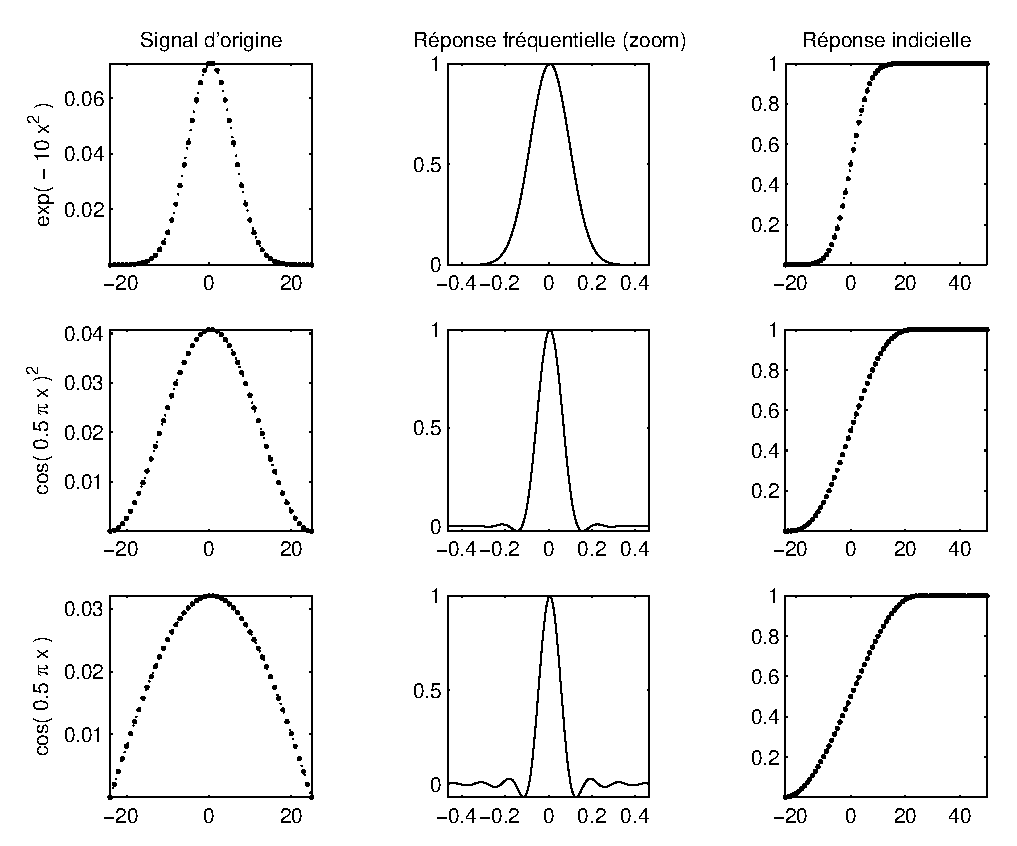
\includegraphics[scale=0.7]{images/diff-types-reponses.eps}
    \end{center}
    \caption{Frequency and index responses}
              \label{fig-diff-types-responses}
\end{figure}
 
 
 
 
 
\begin{rem}{(\upshape \textbf{Time and frequency domain}).} 
\index{Duality!time / frequency} \index{Support!compact} Depending on the answer that interests us, we can see a filter as operating in the time domain (even if the signal is not sampled in time but for example in space) or in the frequency domain. In certain applications, it is natural to create the filter according to the temporal properties which one wants to give to the filter (for example to smooth images in a privileged direction). In other applications, we will be interested in the frequency behavior of the filter (how the filter will remove high frequencies, for a low pass filter at the output of a microphone). The remarks on the time / frequency duality made in Paragraph~\ref{sect2-duality-time-frequency} explain that we cannot have it both ways. For example, if one wishes to create a very precise \textit{bandpass} filter (that is to say with the most compact support possible), it will necessarily be of little use in the time domain, because it will have a very wide impulse response.
\end{rem}
 
 
 
\label{notation-54} Before moving on to the study of two-dimensional filters, let us briefly present an important notion which will be taken up later (during the study of the transform in Z, in Paragraph~\ref{sect1-trans-Z}). This is the notion of \textit{stability} of a filter, which is defined in a very intuitive way.
 
\begin{defn}[Stability]
\index{Stability} A filter $ \Phi^g $ is said to be stable if for any bounded signal $ f \in \CC^\ZZ $, the output $ \Phi^g (\Phi) $ is also bounded.
\end{defn}
A simple calculation shows that
\begin{equation*}
\forall n \in \ZZ, \quad | \Phi^g (f) [n] | \leq \sup_{n \in \ZZ} (| f [n] |) \sum_{k = \minf}^{\pinf}{| g [k] |}.
\end{equation*}
Consequently, for a filter to be stable, it suffices that $ g \in \ell^1 (\ZZ) $, where we have noted $ \ell^1 (\ZZ) $ the space of sequences absolutely summable. We can verify that this condition is also necessary, by taking a sequence $ f $ such that $ f [k] g [-k] = | g [k] | $ (for $ k $ such as $ g [k] \neq $ 0). We then have, if $ g \notin \ell^1 (\ZZ) $,
\begin{equation*}
\Phi^g (f) [0] = \sum_{k = \minf}^{\pinf}{f [k] g [-k]} = \sum_{k = \minf}^{\pinf}{| g [k] |} = + \infty.
\end{equation*}
If $ g \in \ell^1 (\ZZ) $, the filter operator $ \Phi^g $ is a continuous endomorphism of the space of bounded sequences, and its norm is exactly $ \norm{g}_{\ell^1} $.
 
 
The linear filters with finite impulse response which have been considered up to now are therefore always stable. We will see in Paragraph~\ref{sect2-application-trans-z-filters}, that it is possible to build filters which do not have this nice property.
% ------------------------------------------------- -----
% ------------------------------------------------- -----
% sub-section - 2D filtering and image analysis                            
% ------------------------------------------------- -----
% ------------------------------------------------- -----
\subsection{2D filtering and image analysis}
\label{sect2-filtering-2d} 
 
 
\index{Filter!2D} \index{Image smoothing} \index{Image} We can of course consider two-dimensional convolution as it is explained in paragraph \ref{sect2-convolution-2d}. This gives rise to a filter $ \Phi^g $, which acts on two-dimensional signals $ f: \{0, \ldots, \, N-1 \} \times \{0, \ldots, \, N-1 \} \rightarrow \RR $. These signals can be represented as images, since in each \textit{pixel} $ (i, \, j) $ of the image, we have a light intensity $ f [i, \, j] $. More precisely, we most often restrict the end set to a finite set, for example $ \{0, \ldots, \, 255 \} $. These $ 256 $ values represent the famous \textit{levels of gray} which will be displayed on the screen.
 
 
To \guill{smooth} an image, we will once again consider transfer functions $ g $ tightened around $ 0 $, for example a Gaussian:
\begin{equation*}
\forall (k, \, l) \in \{- N / 2, \ldots, \, N / 2 \}^2, \quad g [k, \, l] = \frac{1}{M} \exp \left(- \frac{(2 k / N)^2 + (2 l / N)^2}{2t} \right).
\end{equation*}
The parameter $ M $ is as in the 1D case chosen such that $ \norm{g}_1 = 1 $, and $ t $ is adjusted according to the power of the desired smoothing. Figure \figref{fig-Gaussian-filter-2} shows different Gaussian kernels (top row) as well as an image smoothed by these same Gaussian kernels (bottom row). \begin{figure}[ht]
    \begin{center}
    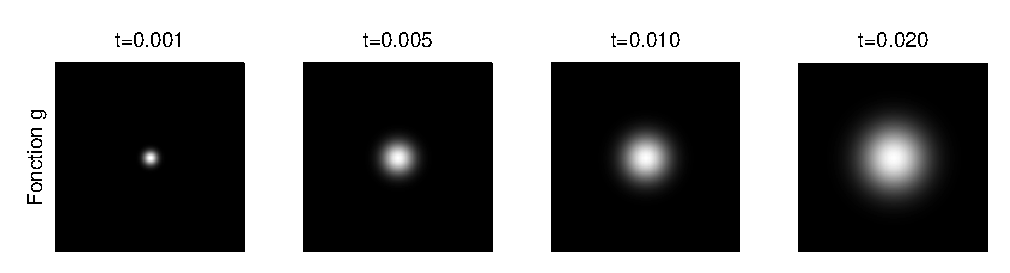
\includegraphics[scale=0.7]{images/filtre-gaussien-1.eps}
    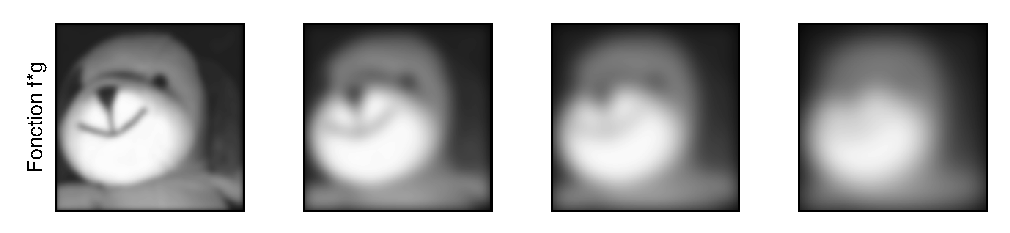
\includegraphics[scale=0.7]{images/filtre-gaussien-2.eps}
    \end{center}
    \caption{Smoothing of an image by a 2D Gaussian}
              \label{fig-Gaussian-filter-2}
\end{figure}
 
 
 
A very common application of image filtering is to soften the noise present in a degraded natural image. This is shown in the figure \figref{fig-filter-2d}, where we can see \textit{Maurice} whose image, of poor quality, has been improved by a Gaussian filter. 

\begin{figure}[ht]
    \begin{center}
    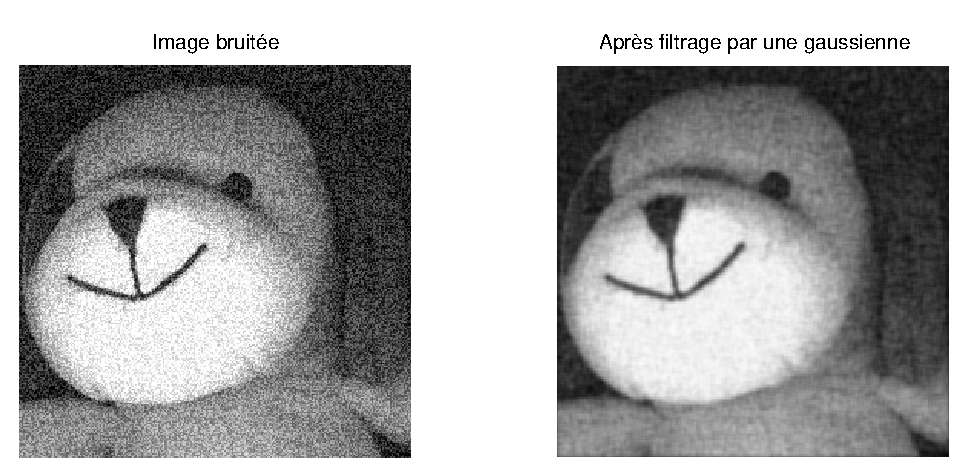
\includegraphics[scale=0.6]{images/filtre-2d.eps}
    \end{center}
    \caption{Image filtering example}
              \label{fig-filter-2d}
\end{figure}

The exercise \oldref{exo-correlation-2d} proposes to go further in image analysis, by applying the correlation calculation to the search for sub-images in a larger image.
% ------------------------------------------------- -----
% ------------------------------------------------- -----
% ------------------------------------------------- -----
% section - Geometric aspects of filtering                            
% ------------------------------------------------- -----
% ------------------------------------------------- -----
% ------------------------------------------------- -----
\section{Geometric aspects of filtering}
% \addcontentsline{toc}{section}{Geometric aspects of filtering}
\label{sect1-aspect-geometriques} 
 
In this section, we will approach the problem of filtering a signal from an original and simple angle, that of plane geometry. Rather than considering the signal studied as a series of values spaced in time, we will use it to describe a polygon drawn in the complex plane. We will then focus on the action of a filter on the shape of this polygon. More precisely, we will see how the successive iterates of the filtered polygon behave.
% ------------------------------------------------- -----
% ------------------------------------------------- -----
% sub-section - Polygon filtering                            
% ------------------------------------------------- -----
% ------------------------------------------------- -----
\subsection{Polygon filtering}
\label{sect2-filtering-polygons} 
 
 
\index{Polygon} \index{Filter!of polygons} In the rest of this talk, we will consider a polygon with $ N $ vertices, $ \Pi $, which we will see as a vector $ \Pi \in \CC^N $. Thus, $ \Pi [0] $ will represent the first vertex of the polygon, $ \Pi [1] $ the second, and so on. Equivalently, we can also consider a polygon as a function $ \Pi: \ZZ/N \ZZ \rightarrow \CC $. This description is very convenient, since it adapts well to the concept of closed polygon. Indeed, we consider that the vertex $ \Pi [i] $ is linked to the vertex $ \Pi [i + 1] $, and we naturally want to link the vertex $ \Pi [N-1] $ to the vertex $ \Pi [0] $. This amounts to considering a $ N $ -periodic signal.
 
 
\index{Iteration} We are interested in the action of a circular filter $ \Phi^g $ on a polygon $ \Pi $. We will therefore consider the iterated polygons $ \Pi^{(k)} $, for $ k \geq 0 $, which are defined as follows:
\begin{equation}
\label{eq-filtering-polygons}
\left\{\begin{array}{ll} \Pi^{(0)} = \Pi & \\\Pi^{(k)} = g * \Pi^{(k-1)} & \forall k> 0 \end{array} \right. ,
\end{equation}
where $ g $ is the filter transfer function. The natural question is to know if $ \Pi^{(k)} $ will tend towards a certain limit polygon, $ \Pi^{(\infty)} $, if the iterated polygons will remain bounded, or if on the contrary they will \guill{explode}. To carry out this study, it suffices to calculate the Fourier transform of the iteration relation \eqref{eq-filtering-polygons}, and we see that
\begin{equation*}
\forall k \geq 0, \quad \wh{\Pi^{(k)}} = (\wh{g})^n \cdot \wh{\Pi}.
\end{equation*}
The study of the convergence of $ \Pi^{(k)} $ is therefore very simple in the Fourier domain. Moreover, thanks to the inversion formula of the transform, a convergence in the Fourier domain is equivalent to a convergence of the polygon. Here are the different cases that can arise. \begin{rs}
\item If $ \exists i \in \{0, \ldots, \, N-1 \} $ such that $ | \wh{g}[i] | > $ 1: then the iterated polygons will explode. This corresponds to cases (a) and (b) in figure \figref{fig-filter-polygons-1}.
\item If for all $ i $, we have either $ | \wh{g}[i] | <1 $ or $ \wh{g}[i] = 1 $, then the iterated polygons will converge to a polygon $ \Pi^{(\infty)} $ which is defined by
\begin{equation*}
\forall i = 0, \ldots, \, N-1, \quad \wh{\Pi^{(\infty)}}[i] = \left\{\begin{array}{lll} 0 & \text{si} & | \wh{g}[i] | <1 \\\wh{\Pi}[i] & \text{si} & \wh{g}[i] = 1 \end{array} \right. .
\end{equation*}
This corresponds to case (c) of figure \figref{fig-filter-polygons-1}.
\item If $ \forall i \in \{0, \ldots, \, N-1 \}, \; | \wh{g}[i] | \leq 1 $, but there is a $ i $ such that $ | \wh{g}[i] | = 1 $ and $ \wh{g}[i] \neq 1 $, then the iterated polygons will not converge, but they will remain bounded. This corresponds to case (d) of figure \figref{fig-filter-polygons-1}. We can notice that if $ \wh{g}[i] $ is a root of unity, then the motion is periodic (even if the phenomenon is difficult to study numerically because of the rounding errors).
\end{rs} 

\begin{figure}[ht] 
    \begin{center}
    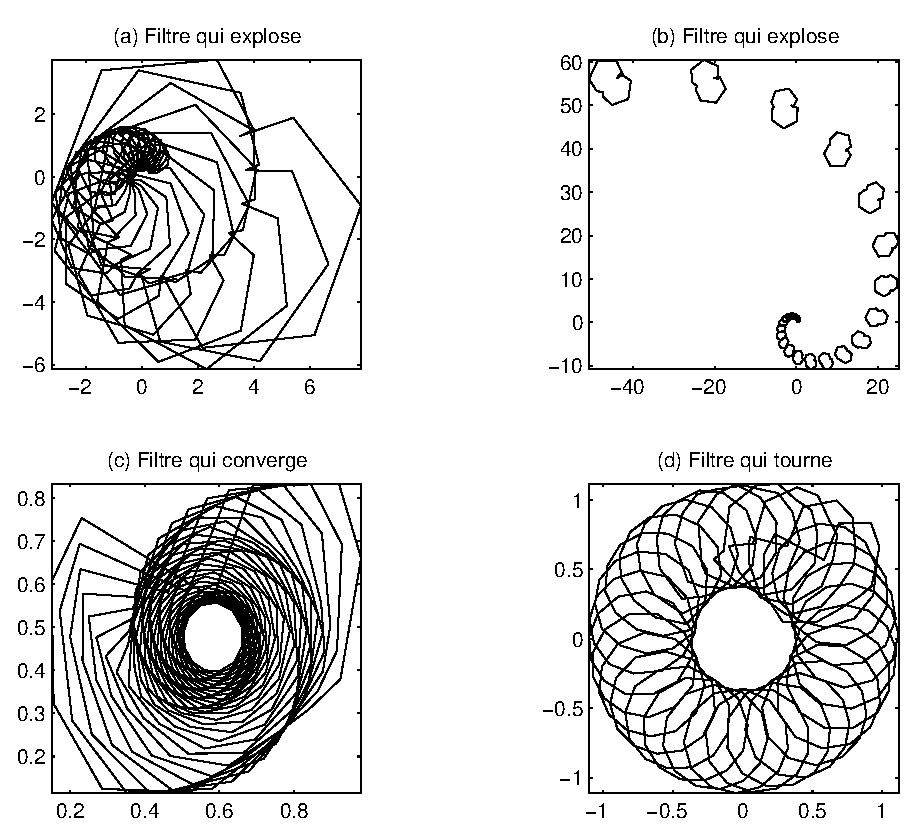
\includegraphics[scale=0.6]{images/filtre-polygones-1.eps}
    \end{center}
    \caption{Different cases of polygon filtering}
              \label{fig-filter-polygons-1}
\end{figure}

Two typical examples of polygon filtering can be given. They are shown in figure \figref{fig-filter-polygons-2}.
 
\begin{exmp}
\index{Center!of gravity} The first corresponds to the filter
\begin{equation*}
g = \{1/2, \, 1/2, \, 0, \ldots, \, 0 \}.
\end{equation*}
This consists of replacing the polygon $ \Pi $ by the polygon $ \Pi^{(1)} $ such that
\begin{equation*}
\Pi^{(1)}[i] = \frac{1}{2} \left(\Pi [i] + \Pi [i + 1] \right).
\end{equation*}
In a way, this amounts to joining the consecutive midpoints on each side of the polygon. Intuitively (and on the drawing of figure \figref{fig-filter-polygons-1}, on the left), one has the impression that the iterated polygons converge towards the center of the polygon. Let's confirm this by calculation:
\begin{equation*}
\wh{g}[k] = \frac{1}{2} \left(1 + e^{- \frac{2 \imath \pi}{N} k} \right) = \cos \left(\frac{k \pi}{N} \right) e^{- \frac{\imath \pi}{N} k}.
\end{equation*}
As we have $ \wh{g}[0] = 1 $ and for $ k \geq 1, \; | \wh{g}[k] | <1 $, we therefore conclude that the iterated polygons will converge to the point $ \wh{\Pi}[0] $, which corresponds to the center of gravity of the polygon.
\end{exmp}
 
 
\begin{exmp}
For the second example, this is a filter which acts in the Fourier domain as follows:
\begin{equation*}
\wh{g} = \{0.8, \, 1, \, 0.8, \ldots, \, 0.8 \}.
\end{equation*}
The iterated polygons will therefore converge to a polygon $ \Pi^{(\infty)} $ such that
\begin{equation*}
\wh{\Pi^{(\infty)}} = \{0, \, \wh{\Pi}[1], \, 0, \ldots, \, 0 \}.
\end{equation*}
We check that this corresponds to a regular polygon inscribed in a circle of radius $ | \wh{\Pi}[1] | $, as we can see in the figure \figref{fig-filter-polygons-2} (right).
\end{exmp}

\begin{figure}[ht] 
    \begin{center}
    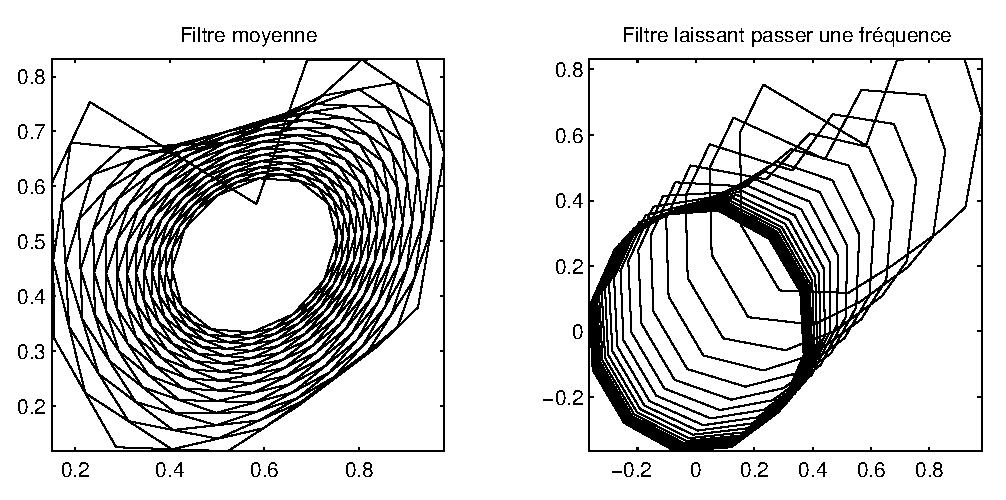
\includegraphics[scale=0.6]{images/filtre-polygones-2.eps}
    \end{center}
    \caption{Average filtering and frequency pass filtering}
              \label{fig-filter-polygons-2}
\end{figure}
 
% ------------------------------------------------- -----
% ------------------------------------------------- -----
% sub-section - Polygonal inequalities                            
% ------------------------------------------------- -----
% ------------------------------------------------- -----
\subsection{Polygonal inequalities}
 
 
\index{Inequality!polygonales} This paragraph is taken from the book by \nompropre{Terras} \cite{terras}. I wanted to insert it into a more general study of geometrical Fourier analysis, which is the subject of this paragraph. The idea is to use the Fourier transform in order to demonstrate inequalities of Euclidean nature on the polygons. The main tool will be the Plancherel equality \ref{prop-formula-floorel-tfd}, which will make it possible to demonstrate the inequalities by passing through the Fourier domain.
 
 
As in the previous paragraph, we consider a polygon $ \Pi $ with $ N $ sides, which can be seen as a function $ \Pi: \ZZ/N \ZZ \rightarrow \CC $. We will define several quantities related to this polygon. First, the sum of the squares of the lengths of the sides:
\begin{equation*}
S (\Pi) \eqdef \sum_{i = 0}^{N-1}{| \Pi [i + 1] - \Pi [i] |^2}.
\end{equation*}
\index{Distance} Then, the sum of the squares of the distances to the center of gravity of the polygon:
\begin{equation*}
T (\Pi) \eqdef \sum_{i = 0}^{N-1}{| \Pi [i] - \wh{\Pi}[0] |^2}.
\end{equation*}
Finally, the oriented area of the polygon:
\begin{equation*}
A (\Pi) \eqdef \frac{1}{2} \sum_{i = 0}^{N-1}{\imagp \left(\ol{\Pi [i]} \Pi [i + 1] \right)}.
\end{equation*}
 
 
\begin{prop}
We have the following inequalities: \begin{itemize}
\item [{\upshape (i)}] $ A (\Pi) \leq \frac{1}{2} T (\Pi) $
\item [{\upshape (ii)}] $ 4 \sin^2 \left(\frac{\pi}{N} \right) T (\Pi) \leq S (\Pi) $.
\end{itemize}
\end{prop}
\begin{proof}
\index{Offset operator} \textbf{Inequality (i)}: We introduce the offset operator $ T $ defined by the relation $ T \Pi [k] = \Pi [k + 1] $, which lets write
\begin{equation*}
A (\Pi) = \frac{1}{2} \imagp \left(\sum_{k = 0}^{N-1}{\Pi [i] \ol{T \Pi [i]}} \right).
\end{equation*}
Then just use Plancherel's formula to calculate $ A (\Pi) $ in the Fourier domain:
\begin{equation*}
A (\Pi) = \frac{1}{2} \imagp \left(\sum_{k = 0}^{N-1}{\wh{\Pi}[k] \ol{\Ff(T \Pi) [k]}} \right).
\end{equation*}
We then use the fact that $ \Ff(T \Pi) [k] = e^{\frac{2 \imath \pi}{N} k} \wh{\Pi}[k] $ to get
\begin{equation*}
A (\Pi) = \frac{1}{2} \sum_{k = 0}^{N-1}{\sin \left(\frac{2 k \pi}{N} \right) | \wh{\Pi}[k] |^2}.
\end{equation*}
By noting that $ \sin \left(\frac{2 k \pi}{N} \right) \leq 1 $, we do obtain the desired inequality, after having once again used the Plancherel formula. \\\textbf{Inequality (ii)}: To do this, let's introduce the filter whose transfer function is equal to $ g \eqdef \{- 1, \, 1, \, 0, \ldots, \, 0 \} $ . We can rewrite the quantity $ S (\Pi) $ as follows:
\begin{equation*}
S (\Pi) = \sum_{k = 0}^{N-1}{| g * \Pi [k] |^2} = \frac{1}{N} \sum_{k = 0}^{N-1}{\left| \Ff(g * \Pi) [k] \right|^2}.
\end{equation*}
For the last tie, we used Plancherel's formula. Let us calculate the modulus of the Fourier transform of $ g $:
\begin{equation*}
\forall k = 1, \ldots, \, N-1, \quad | \wh{g}[k] |^2 = | e^{- \frac{2 \imath \pi}{N} k} - 1 |^2 = 4 \sin^2 \left(\frac{k \pi}{N} \right) \geq 4 \sin^2 \left(\frac{\pi}{N} \right).
\end{equation*}
It only remains to use the convolution property to get, like $ \wh{g}[0] = 0 $,
\begin{equation*}
S (\Pi) = \frac{1}{N} \sum_{k = 1}^{N-1}{| \wh{g}[k] |^2 | \wh{\Pi}[k] |^2} \geq \frac{1}{N} 4 \sin^2 \left(\frac{\pi}{N} \right) \sum_{k = 1}^{N-1}{| \wh{\Pi}[k] |^2}.
\end{equation*}
We then conclude by using Plancherel's formula once again:
\begin{equation*}
\frac{1}{N} \sum_{k = 1}^{N-1}{| \wh{\Pi}[k] |^2} = \frac{1}{N} \sum_{k = 0}^{N-1}{\left| \Ff \left(\Pi [k] - \wh{\Pi}[0] \right) \right|^2} = T (\Pi).
\end{equation*}
Which ends the demonstration.
\end{proof}
 
% ------------------------------------------------- -----
% ------------------------------------------------- -----
% sub-section - Fourier descriptors                            
% ------------------------------------------------- -----
% ------------------------------------------------- -----
\subsection{Fourier descriptors}
 
 
\index{Pattern recognition} To end this chapter on the applications of Fourier theory to geometry, we will tackle the problem of \textit{pattern recognition}. To be more precise, we want to know if two polygons $ \Pi_1 $ and $ \Pi_2 $ represent the same shape, up to translation, rotation and homothety. We will of course try to compare the two Fourier transforms $ \wh{\Pi}_1 $ and $ \wh{\Pi}_2 $.
 
 
It is therefore a question, from a transformed vector, of creating a quantity $ \Dd (\Pi) $ characterizing a polygon $ \Pi $ up to translation and similarity. Here are the three operations to perform: \begin{rs}
\item \index{Translation} for the translation: we know that only the component $ \wh{\Pi}[0] $ is modified by a translation. In fact, $ \wh{\Pi}[0] $ precisely represents the center of gravity of the polygon. We will therefore purely and simply ignore the first entry of the transformed vector.
\item \index{Rotation} \index{Homothety} \index{Similarity} for rotation and homothety: we consider a plane similarity with center $ \omega $, of angle $ \theta $, and of ratio $ r $. This corresponds to the transformation $ z \mapsto \omega + re^{\imath \theta} (z - \omega) $. We check that this transformation changes the Fourier coefficients $ \wh{\Pi}[k] $ (for $ k> 0 $) by multiplying them by $ re^{\imath \theta} $. Suppose that $ \wh{\Pi}[1] \neq 0 $ (otherwise, we take another index $ k_0> 0 $ such as $ \wh{\Pi}[k_0] \neq 0 $). To cancel the effect of the homothety, it suffices to consider the quantities $ \frac{\wh{\Pi}[2]}{\wh{\Pi}[1]}, \, \frac{\wh{\Pi}[3]}{\wh{\Pi}[1]}, \ldots, \, \frac{\wh{\Pi}[N-1]}{\wh{\Pi}[1]} $.
\item for the invariant by circular shift of the data: we want the polygon $ \Pi'\eqdef T \Pi $ defined by $ \Pi' = \{\Pi [1], \, \Pi [2], \ldots, \, \Pi [N-1], \, \Pi [0] \} $ is indistinguishable from the polygon $ \Pi $, which means that $ \Dd (\Pi) = \Dd (\Pi' ) $. We see that $ \wh{\Pi'}[k] = e^{\frac{2 \imath \pi}{N} k} \wh{\Pi}[k] $. To have this invariance, we will therefore consider the modulus of the quantities already calculated.
\end{rs} After all these observations, we are therefore led to assign to each polygon $ \Pi $ a Fourier descriptor, which we define as follows.
 
\begin{defn}[Fourier descriptor]
\index{Fourier descriptor} Let $ \Pi $ be a polygon with $ N $ sides such that $ \wh{\Pi}[1] \neq 0 $. Its Fourier descriptor $ \Dd (\Pi) $ is a complex vector of size $ N-2 $ defined as follows:
\begin{equation*}
\Dd (\Pi) \eqdef \left\{\frac{| \wh{\Pi}[2] |}{| \wh{\Pi}[1] |}, \, \frac{| \wh{\Pi}[3] |}{| \wh{\Pi}[1] |}, \ldots, \, \frac{| \wh{\Pi}[N-1] |}{| \wh{\Pi}[1] |} \right\}.
\end{equation*}
\index{Distance!between polygons} We then define the distance between two polygons (we suppose that they verify $ \wh{\Pi}_i [1] \neq 0 $) $ \Pi_1 $ and $ \Pi_2 $ of the following way:
\begin{equation*}
d (\Pi_1, \, \Pi_2)^2 \eqdef \sum_{k = 0}^{N-3}{\left(\Dd (\Pi_1) [k] - \Dd (\Pi_2) [k] \right)^2}.
\end{equation*}
\end{defn}
Two polygons $ \Pi_1 $ and $ \Pi_2 $ which are images of each other by a plane similarity therefore verify $ d (\Pi_1, \, \Pi_2) = 0 $. However, we should be careful that the converse is false. Indeed, if we choose arbitrary numbers $ \theta_0, \ldots, \, \theta_{N-1} $, then the polygon $ \Pi_2 $ defined by $ \wh{\Pi}_2 [k] \eqdef e^{\imath \theta_k} \wh{\Pi}_1 [k] $ checks $ d (\Pi_1, \, \Pi_2) = 0 $. In practice however, the value of $ d $ gives a good idea of the similarity between two forms. This is illustrated in the figure \figref{fig-fourier-descriptors}, where the second polygon is close to the first.
% ------------------------------------------------- -----
% ------------------------------------------------- -----
% ------------------------------------------------- -----
% section - Numerical solution of derivative equations by \-tials                            
% ------------------------------------------------- -----
% ------------------------------------------------- -----
% ------------------------------------------------- -----
\section{Numerical solution of derivative equations by \-tials}
% \addcontentsline{toc}{section}{Numerical solution of derivative equations by \-tials}
\label{sect1-resolution-edp} 
 
 
 
\index{Partial Differential Equation} One of the main utilities of the continuous Fourier transform is the solution of partial differential equations. From a purely formal point of view (almost completely algebraic), it allows to replace a complex problem (a linear differential equation) in a much simpler problem, a polynomial equation. This is because the Fourier transform replaces the derivation with respect to $ x $ in multiplication by $ \imath x $. Of course, you have to worry about the convergence problems as well as the boundary conditions, but the Fourier transform turns out to be a very powerful theoretical tool to demonstrate the existence of solutions for many equations. \begin{figure}[ht ]
    \begin{center}
    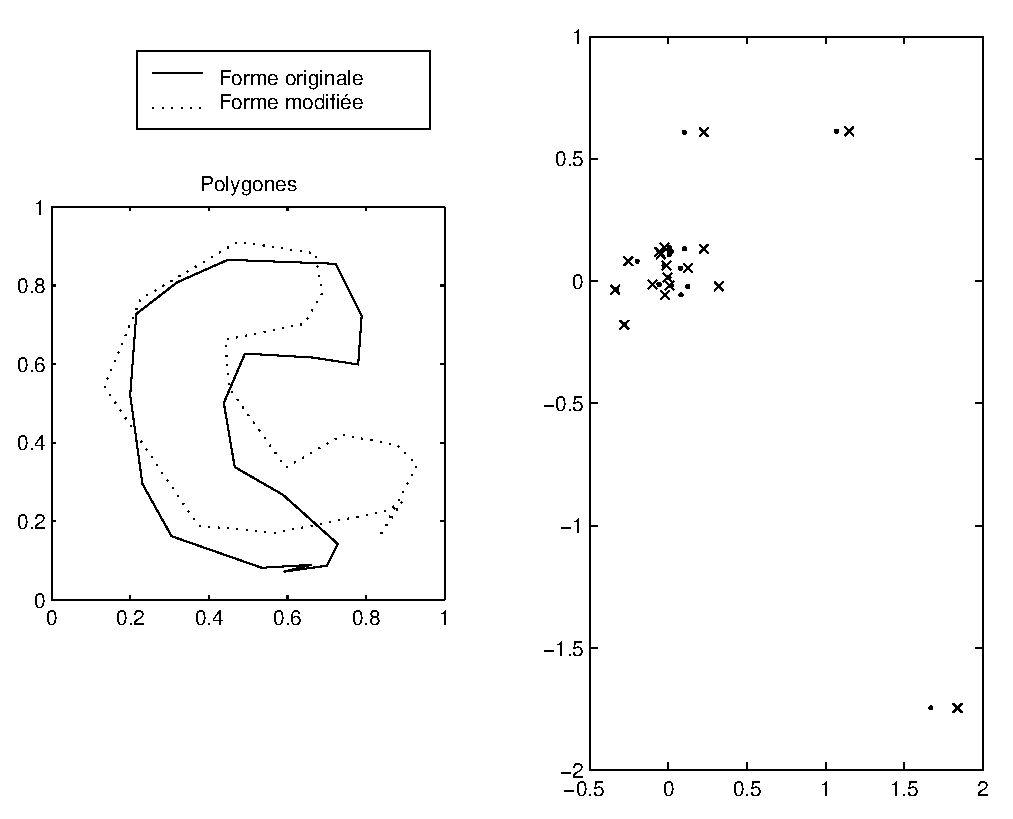
\includegraphics[scale=0.6]{images/fourier-descriptors.eps}
    \end{center}
    \caption{Fourier descriptors for two similar forms}
              \label{fig-fourier-descriptors}
\end{figure}
 
 
 
From a practical point of view, the numerical computation of the solution of an equation can, at various times of the discretization process, lead to the use of the discrete Fourier transform. This can come from a pure and simple discretization of the continuous Fourier transform (for example for \textit{the heat equation}, paragraph \ref{sect2-resol-eq-heat}), or from a more ingenious way to simplify and speed up calculations (for example for \textit{Poisson's equation}, paragraph \ref{sect2-resol-eq-Poisson}). In the following paragraphs, we will focus on these numerical aspects; The theoretical use of the continuous transform is detailed in particular in the exercise \oldref{exo-unicite-eq-heat}.

% ------------------------------------------------- -----
% ------------------------------------------------- -----
% sub-section - Calculation of Fourier coefficients                            
% ------------------------------------------------- -----
% ------------------------------------------------- -----
\subsection{Calculation of Fourier coefficients}
\label{sect2-calcul-coef-fourier} 
 
 
\index{Fourier coefficient!calculation by FFT} As we saw in paragraph \ref{sect2-calculus-trans-fourier-approach}, the FFT algorithm allows to calculate in an approximate way the value of the Fourier transform continue at certain frequencies $ \xi_k $. But in reality, the calculation of $ \wh{f}[\xi_k] $ that we carried out corresponds to the approximation of the integral:
\begin{equation}
\label{eq-lien-fft-calcul-coef-fourier}
\wh{f} (\xi_k) \approx \Delta \int_{0}^{N \Delta}{f(t) e^{- \frac{2 \imath \pi}{N \Delta} kt} \d t}.
\end{equation}
Now, if we denote by $ f_1 $ the periodic function of period $ N \Delta $ which coincides with $ f $ on the interval $ [0, \, N \Delta] $, the equation \eqref{eq-lien-fft-calcul-coef-fourier} corresponds to the calculation of $ c_k (f_1) $, the $ k^{ieme} $ Fourier coefficient of the function $ f_1 $.
 
 
Let us summarize all these results by a formula allowing to calculate in an approximate way $ N $ Fourier coefficients for a periodic function $ f $ of period $ 1 $:
\begin{equation*}
\forall n \in \{-N / 2 + 1, \ldots, \, 0, \ldots, \, N / 2 \}, \quad c_n (f) \eqdef \int_0^1{f(t) e^{- 2 \imath \pi nt} \d t} \approx \frac{1}{N} \wh{f}[n],
\end{equation*}
where we denote by $ \wh{f} $ the transformed Fourier vector of the vector $ \{f(k / N) \}_{k = 0}^{N-1} $.
 
 
The FFT algorithm will therefore allow the calculation of $ N $ Fourier coefficients of a function sampled in $ N $ points all at once. Moreover, the techniques of adding zeros and refining the sample make it possible to modulate the number of coefficients calculated for the same sample. The only potential problem lies in the lack of precision (the rectangle method is only of order 1), which can be problematic when the Fourier coefficients decrease rapidly towards 0, as is the case for a very regular function. Two solutions are then possible: \begin{rs}
\item increase the number of interpolation points.
\item use a higher integration method. It is possible to show a discrete Fourier transform with formulas other than that of rectangles (for example that of \textit{Simpson}). The exercise \oldref{exo-calcul-approaches-transfo-frac}, question 2, details this technique.
\end{rs}
% ------------------------------------------------- -----
% ------------------------------------------------- -----
% sub-section - Application to the heat equation                            
% ------------------------------------------------- -----
% ------------------------------------------------- -----
\subsection{Application to the heat equation}
\label{sect2-resol-eq-heat} 
 
 
\index{Fourier@\nompropreindex{Fourier}} In this paragraph, we will apply the method described in the previous paragraph, which allows us to calculate all at once a very large number of Fourier coefficients (admittedly with questionable precision). It is a question of solving the heat equation, which historically had a very important role, since it was this which pushed \nompropre{Joseph Fourier} to develop his theory, in his article \textit{Theorie Analytique de the Heat} (1822).
 
 
\index{Equation!of heat} We want to solve in an approximate way the equation of heat on the circle $ S^1 \eqdef \RR / \ZZ $:
\begin{equation}
\label{heat-eq}
\left\{\begin{array}{l} \forall (t, \, x) \in \RR_*^{+} \times S^1, \quad \displaystyle{\pd{u}{t} = \kappa \pdd{u}{x}} \\\forall x \in S^1, \quad u (0, \, x) = f(x) \end{array} \right. ,
\end{equation}
where the sought solution $ u $ is assumed to be sufficiently regular over $ \RR_*^{+} \times S^1 $, and continues over $ \RR^{+} \times S^1 $. In this paragraph, we are not going to use a finite difference method, unlike what we will do in the \ref{sect2-resol-eq-Poisson} paragraph to solve the Poisson equation. The exercise \oldref{exo-resol-eq-heat-diff-finies} studies the stability of such a method for the heat equation. Instead, we will explicitly solve the continuous equation, and calculate approximations of the solution by FFT.
 
 
This equation reflects the evolution of heat in a circle of length 1, completely isolated, and of which we know the initial temperature distribution. The constant $ \kappa $ translates the conductivity of the material, and without loss of generality, it will be taken equal to $ \frac{1}{2} $ in the following. Indeed, we can replace the function $ u $ by $ (t, \, x) \mapsto u \left(\frac{t}{2 \kappa}, \, x \right) $, which does not modify the problem. For an exposition on the different applications of series and the Fourier transform to differential equations (and in particular to the heat equation), the book of \nompropre{Dym} and \nompropre{MacKean} \cite{dym} is an excellent source. In the following, we will content ourselves with stating the main results. In particular, the uniqueness result is detailed in the exercise \oldref{exo-unicite-eq-heat}.
 
 
\index{Fourier!series} To begin with, we are looking for a formal solution in the form
\begin{equation*}
u (t, \, x) \eqdef \sum_{n \in \ZZ}{c_n (t) e_n (x)} \quad \quad \text{with} \quad e_n (x) \eqdef e^{2 \imath \pi nx},
\end{equation*}
since intuitively, the solution must be periodic at $ t $ fixed. The coefficients $ c_n (t) $ are defined by
\begin{equation*}
\forall t> 0, \quad c_n (t) \eqdef \int_0^1{u (t, \, x) e_n (-x)} \d x.
\end{equation*}
By doing two integrations by parts, we obtain a differential equation verified by $ c_n $:
\begin{equation*}
\begin{split}
\frac{d c_n}{dt} (t) = & \int_0^1{\pd{u}{t} (t, \, x) e_n (-x) \d x} = \int_0^1{\frac{1}{2} \pdd{u}{x} (t, \, x) e_n (-x) \d x} \\
= & - 2 \pi^2 n^2 \int_0^1{u (t, \, x) e_n (-x) \d x} = -2 \pi^2 n^2 c_n (t).
\end{split}
\end{equation*}
As $ c_n (0) = \wh{f} (n) $ (the \ordin{n}{th} Fourier coefficient of $ f $), we obtain a formal solution of the heat equation \eqref{heat-eq}:
\begin{equation}
\label{eq-solution-heat-equation}
\forall (t, \, x) \in \RR_*^{+} \times S^1, \quad u (t, \, x) = \sum_{n \in \ZZ}{\wh{f} (n) \exp (-2 \pi^2n^2 t) e_n (x)}.
\end{equation}
The fact that the function $ u $ thus defined is indeed the solution of the problem posed for $ t> 0 $ comes from the fact that we can differentiate under the sum sign because the series of terms $ \exp (-2 \pi^2n^2 t) $ is normally convergent for $ t \geq \epsilon> 0 $, as well as all its derivatives with respect to $ t $. The only thing difficult to show is that we have
\begin{equation*}
\norm{u (t, \, \cdot) - f}_{\infty} \tv{t \to 0} 0,
\end{equation*}
that is to say that the initial conditions are well respected. We recall that $ \norm{\cdot}_\infty $ denotes the uniform norm over $ S^1 $. All this is detailed in the exercise \oldref{exo-unicite-eq-heat} at the same time as the proof of the uniqueness of the solution.
 
\begin{rem}{(\upshape \textbf{Continuous filtering}).} 
\index{Filter!continuous} \index{Gaussian} Intuitively, the passage from $ u (0, \, \cdot) = f $ to $ u (t, \, \cdot) $ corresponds to the multiplication of the coefficients of Fourier $ \wh{f} (n) $ of $ f $ by $ \exp (-2 \pi^2n^2 t) $. This amounts to filtering $ f $ by a Gaussian, that is to say to smooth the starting function. The larger $ t $, the greater the variance of the Gaussian, and therefore the more pronounced the blurring effect induced by the filtering. Ultimately, when $ t \rightarrow + \infty $, the filtering simply corresponds to averaging the function, so the heat distribution is uniform.
\end{rem}
 
 
 
In order to approximate the solution $ u $ of the heat equation, we will, for some fairly large $ N $ fixed (which we assume to be a power of 2), calculate
\begin{equation*}
u_N (t, \, x) \eqdef \sum_{n = -N / 2}^{N / 2-1}{c_n (t) e_n (x)}.
\end{equation*}
\index{Matlab@\Matlab{}} Of course, we will use the technique developed in paragraph \ref{sect2-calcul-coef-fourier} and therefore sample the function $ f $ according to a vector $ \wt{f} \eqdef \{f(k / n) \}_{k = 0}^{N-1} $. The calculation of the FFT of this vector allows us, up to a factor $ \frac{1}{N} $, to calculate approximately $ N $ Fourier coefficients of the function $ f $, and therefore to construct the function $ u_N $. All this is detailed in the \Matlab{} programs presented in the \annexeref{sect1-listing-heat} paragraph. The only technical difficulty is that the Fourier coefficients calculated by the FFT are not arranged in the right order, but via the indexing $ \{0, \ldots, \, N / 2-1, \, -N / 2 , \ldots, \, -1 \} $. We can see the evolution of the solution over time in the figure \figref{fig-eq-heat-evolution}, where the initial data is an indicator function (therefore discontinuous). We can clearly see the regularizing effect of the heat equation: for $ t> 0 $, the solution becomes smooth, and tends towards a constant function when $ t $ tends towards $ + \infty $. \begin{figure}[ht]
    \begin{center}
    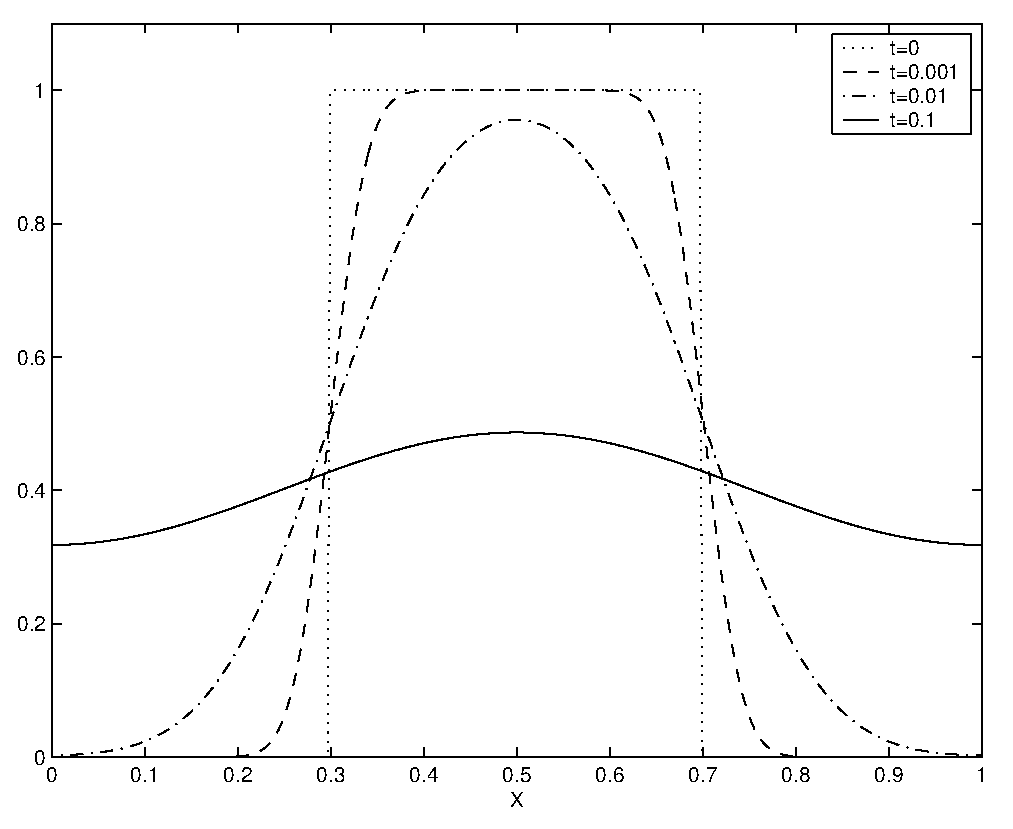
\includegraphics[scale=0.4]{images/eq-chaleur-evolution.eps}
    \end{center}
    \caption{Evolution of the solution of the heat equation}
              \label{fig-eq-heat-evolution}
\end{figure}
 
 
\begin{rem}{(\upshape \textbf{Discrete filtering}).} 
\index{Filter!discrete} Solving the heat equation by DFT therefore amounts to performing a discrete filtering with an increasingly strong low-pass filter. In essence, filtering through a symmetrical low pass filter amounts to solving the heat equation for a certain time $ t $. The more the filter is regularizing, the greater $ t $.
\end{rem}
 
% ------------------------------------------------- -----
% ------------------------------------------------- -----
% sub-section - Solving the Poisson equation by finite differences                            
% ------------------------------------------------- -----
% ------------------------------------------------- -----
\subsection{Solving the Poisson equation by finite differences}
\label{sect2-resol-eq-Poisson} 
 
 
\index{Poisson's equation} \index{Poisson@\nompropreindex{Poisson}} We want to find a function $ u: [0, \, 1] \times [0, \, 1] \rightarrow \RR $ sufficiently regular (of class $ \Cc^2 $) which satisfies the equation of \textit{Poisson}:
\begin{equation}
\label{eq-fish}
\left\{\begin{array}{l} \forall (x, \, y) \in [0, \, 1] \times [0, \, 1], \quad \displaystyle{\Delta u (x , \, y) \eqdef \pdd{u}{x} + \pdd{u}{y} = f(x, \, y)} \\\forall x \in [0, \, 1], \quad u (x, \, 0) = u_{x0} (x) \quad \text{and} \quad u (x, \, 1) = u_{x1} (x) \\\forall y \in [ 0, \, 1], \quad u (0, \, y) = u_{0y} (y) \quad \text{and} \quad u (1, \, y) = u_{1y} (y) \end{array} \right.
\end{equation}
where $ f: \RR^2 \rightarrow \RR $ is a continuous function known in advance, and the functions $ u_{x0} $, $ u_{x1} $, $ u_{0y} $ and $ u_{1y} $ are also supposedly known continuous functions (we fix the values of the solution on the edges).
 
 
The equation of \textit{Poisson} has very important interpretations, especially in physics. We can note: \begin{rs}
\item \index{Elastic membrane} \textit{equation of an elastic membrane}: the surface of the membrane is represented by the equation $ z = u (x, \, y) $. The function $ f $ represents the surface amount of forces applied vertically to the surface. Imposing the value of the function $ u $ on the edges corresponds to fixing the edges of the surface to a reinforcement.
\item \index{Electric potential} \textit{equation of an electric potential}: the quantity $ u (x, \, y) $ represents the value of a surface electric potential at a point $ (x, \, y ) $, and the function $ f $ takes into account a surface distribution of electric charges.
\end{rs} \index{Laplace's equation} \index{Laplace@\nompropreindex{Laplace}} \index{Function!harmonic} \index{Difference!finite} In the particular case where the function $ f $ is zero , we speak of the equation of \textit{Laplace}, and the function $ u $ is then called \textit{harmonic function}. Obviously, we show that the real part of a holomorphic function is harmonic. We can even show that locally, the converse is true (and therefore a harmonic function has partial derivatives at any order!). For more details on the theory of harmonic functions, one can consult the book of \nompropre{Rudin} \cite [p.275]{rudin}.
 
 
We propose to approach the solution $ u $ of the equation \eqref{eq-fish} by the method of \textit{finite differences}. To do this, we will discretize the square $ [0, \, 1] \times [0, \, 1] $ according to $ N + 1 $ points on both directions. We therefore seek an approximate solution $ \{U (i, \, j) \}_{0 \leq i, \, j \leq N} $, where $ U (i, \, j) $ represents an approximation of $ u (ih, \, jh) $ (we noted $ h \eqdef \frac{1}{N} $ the step of the subdivision). By replacing the Laplacian $ \Delta u $ by a discrete approximation, we obtain, for the interior squared points, the following equations, for $ i $ and $ j $ in $ \{1, \ldots, \, N-1 \} $,
\begin{equation}
\label{eq-poisson-discretise}
\frac{1}{h^2} \left\{U (i-1, \, j) + U (i + 1, \, j) + U (i, \, j + 1) + U (i , \, j-1) - 4 U (i, \, j) \right\} = F (i, \, j),
\end{equation}
where we denote by $ F (i, \, j) \eqdef f(ih, \, jh) $ the right side of the equation. We have of course paid attention to the boundary terms ($ i, \, j = 0, \, N $), which are not part of the system since they are fixed once and for all by the boundary conditions.
 
 
\index{Filtering} \index{Filter} We would thus be tempted to write the equation \eqref{eq-poisson-discretise} as a convolution by a filter $ \Phi $:
\begin{equation*}
U * \Phi = F
\end{equation*}
\index{Convolution!2D} where $ * $ denotes the 2D circular convolution operator, defined in paragraph \ref{sect2-convolution-2d}, and the transfer function is written
\begin{equation}
\label{eq-filter-eq-fish}
\Phi \eqdef \frac{1}{h^2} \begin{pmatrix} 1 & & & \\& & \vdots & \\& \ldots & 0 & \ldots \\& & \vdots & \\1 & & & \\-4 & 1 & & 1 \\\end{pmatrix},
\end{equation}
(it should be remembered that the functions considered are N periodic, so that the negative frequencies are pushed to the other end of the table). However, there are at least two objections to this writing. \begin{rs}
\item The filters operate on a periodic signal, but this is not the case here: the values of the edges have no reason to \guill{re-stick}. Moreover, the equation \eqref{eq-poisson-discretise} is only valid inside the domain, that is to say for $ 0 <i, \, j <N $. It does not describe a circular convolution.
\item The edge values are taken into account in the filtering, so they are part of the unknowns: on the contrary, we want them to be fixed.
\end{rs} To work around this problem, it suffices to make null $ U $ at the ends, that is to say for $ i, \, j = 0, \, N $, quite simply by passing in the right-hand side the edge terms. Here is for example an equation obtained for $ i = 1 $ and $ 1 <j <N-1 $:
\begin{equation*}
\begin{split}
\frac{1}{h^2} \left\{0 + U (2, \, j) + U (1, \, j + 1) + U (1, \, j-1) - 4 U ( 1, \, j) \right\} & = F (i, \, j) - \frac{1}{h^2} u_{0y} (jh) \\
& \eqdef \wt{F} (i, \, j),
\end{split}
\end{equation*}
(we used the fact that $ U (0, \, j) = u_{0y} (jh) $ the value fixed on the edge $ x = 0 $). By doing the same for the four edges of the matrix $ F $, we create a new matrix $ \wt{F} $ zero on the edges, and thanks to this manipulation, we can replace the unknown $ U $ by an unknown $ \wt{U} $ which is zero on the edges. It remains precisely to solve the problem of the application of the filter on the edges (the equation \eqref{eq-poisson-discretise}) is only valid inside). To be able to do this, it suffices to extend the functions considered by imparity along the two axes. Indeed, the nullity of the function on the edges as well as the equation \eqref{eq-poisson-discretise} of the filter shows that the terms symmetrical with respect to an edge must be of opposite signs. For example, we have the equation
\begin{equation*}
U (1, \, j) + U (-1, \, j) = \wt{F} (0, \, j) = 0,
\end{equation*}
hence $ U (1, \, j) = - U (-1, \, j) $. We therefore extend the matrices $ \wt{U} $ and $ \wt{F} $ to obtain matrices (always noted in the same way) of size $ 2 N $ odd. Thus, in the (simplistic, but instructive) case where $ N = 3 $, the matrix $ \wt{F} $ will be written
\begin{equation*}
\wt{F} = \begin{pmatrix} 0 & 0 & 0 & 0 & 0 & 0 \\0 & \wt{F} (1, \, 1) & \wt{F} (2, \, 1 ) & 0 & - \wt{F} (2, \, 1) & - \wt{F} (1, \, 1) \\0 & \wt{F} (1, \, 2) & \wt{F} (2, \, 2) & 0 & - \wt{F} (2, \, 2) & - \wt{F} (1, \, 2) \\0 & 0 & 0 & 0 & 0 & 0 \\0 & - \wt{F} (1, \, 2) & - \wt{F} (2, \, 2) & 0 & \wt{F} (2, \, 2) & \wt{F} (1, \, 2) \\0 & - \wt{F} (1, \, 1) & - \wt{F} (2, \, 1) & 0 & \wt{F} (2, \, 1) & \wt{F} (1, \, 1) \\\end{pmatrix}.
\end{equation*}
With all these new conventions, the equation \eqref{eq-poisson-discretise}, which extends to $ 0 \leq i, \, j \leq 2N $ and is also true as a periodic convolution, is written
\begin{equation*}
\wh{U} * \wt{\Phi} = \wt{F},
\end{equation*}
where $ \wt{\Phi} $ is still defined as in the equation \eqref{eq-filter-eq-fish}, but this time is of size $ 2 N $.
 
 
The idea is then to take the 2D Fourier transform of the two members, since the latter transforms the convolution product into a simple product, as stated in the proposition \ref{sect1-tfd-prod-convol}. We get the very nice equation
\begin{equation*}
\Ff \left(\wt{U} \right) \cdot \Ff \left(\wt{\Phi} \right) = \Ff \left(\wt{F} \right),
\end{equation*}
where we denote by $ \cdot $ the term-to-term product of the two matrices. This equation is now very easy to solve, since we know how to calculate the transform of $ \wt{\Phi} $, as shown by the following lemma.
 
\begin{lem}
The Fourier transform of the transfer function $ \Phi $ is given by
\begin{equation*}
\Ff \left(\wt{\Phi} \right) = - \frac{4}{h^2} \left\{\sin \left(\frac{i \pi}{2N} \right)^2 + \sin \left(\frac{j \pi}{2N} \right)^2 \right\}_{0 \leq i, \, j \leq 2N-1}.
\end{equation*}
\end{lem}
\begin{proofnoqed}
It is enough to apply the definition and to make a grouping of terms:
\begin{align*}
\Ff \left(\wt{\Phi} \right) [i, \, j] & = \sum_{k, \, l}{\Phi [k, \, l] e^{\frac{2 \imath \pi}{2N} ki} e^{\frac{2 \imath \pi}{2N} lj}} \\
& = \frac{1}{h^2} \left\{e^{\frac{2 \imath \pi}{2N} i} + e^{\frac{2 \imath \pi}{2N} j} + e^{- \frac{2 \imath \pi}{2N} i} + e^{- \frac{2 \imath \pi}{2N} j} - 4 \right\} \\
& = - \frac{4}{h^2} \left\{\sin \left(\frac{i \pi}{2N} \right)^2 + \sin \left(\frac{j \pi}{2N} \right)^2 \right\}. \tag*{\qed}
\end{align*}
\end{proofnoqed}
So we get
\begin{equation*}
G (i, \, j) = \Ff \left(\wt{U} \right) (i, \, j) = \frac{\Ff(\wt{F}) (i, \, j)}{\sin^2 \left(\frac{i \pi}{2N} \right) + \sin^2 \left(\frac{j \pi}{2N} \right)},
\end{equation*}
(be careful with the division $ 0 / $ 0 for $ i = j = $ 0, but we know that the result is 0). We finish thanks to the calculation of the inverse transform, $ \wt{U} = \Ff^{-1} (G) $. It only remains to extract the part of the matrix $ \wt{U} $ that interests us (that is to say $ 0 \leq i, \, j \leq N $), and to add the terms that we had cut off at the beginning.
 
 
\index{Matlab@\Matlab{}} The entirety of this method to solve the Poisson equation is taken algorithmically in \Matlab{} in the paragraph \annexeref{sect1-listing-fish}. To be able to observe the quality of the approximation, we chose an equation for which we know the solution (in fact, we first choose the solution, then we calculate the right hand side), and we create the boundary functions accordingly . Figure \figref{fig-eq-fish} shows the solution of a Poisson equation for which we explicitly know a solution, namely $ u (x, \, y) = e^{xy} $. The figure \figref{fig-eq-Poisson-modif} uses the same equation, but modifies the conditions on two of the edges. 

\begin{figure}[ht] 
\begin{minipage}{0.5 \linewidth}
    \begin{center}
    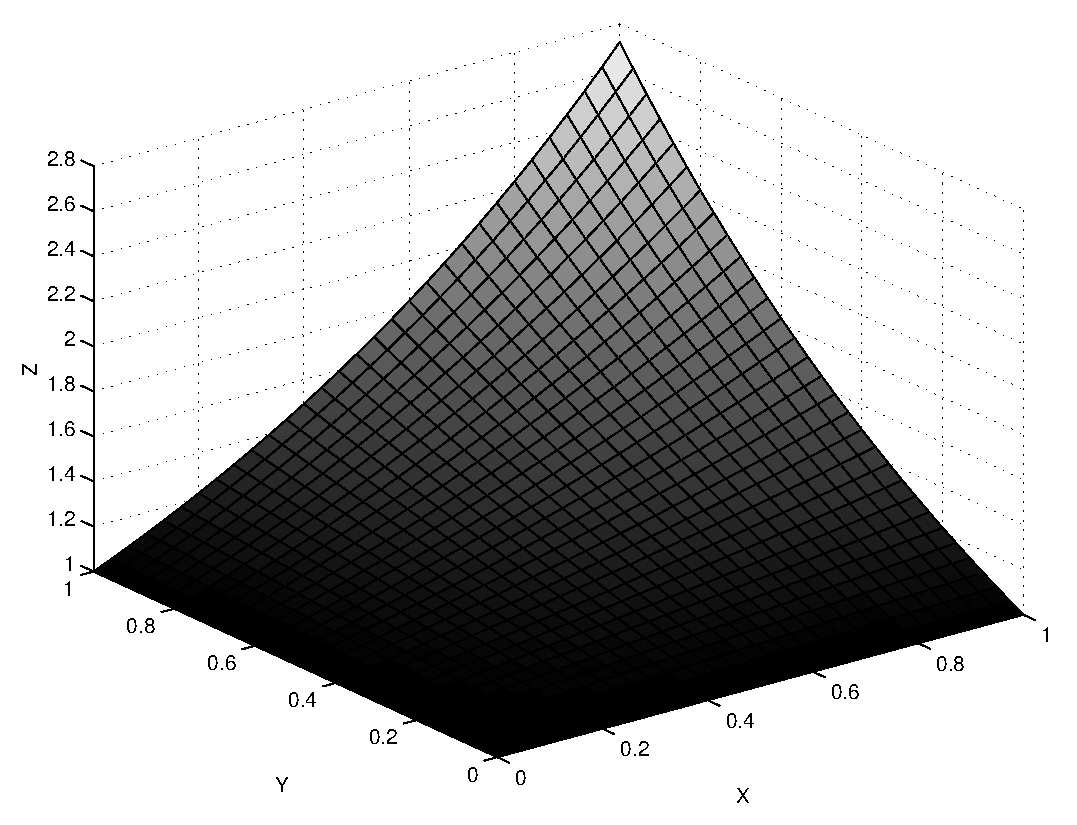
\includegraphics [scale = 0.3]{images/eq-poisson.eps}
    \caption{Solution of the Poisson equation}
              \label{fig-eq-fish}
    \end{center}
\end{minipage}
\begin{minipage}{0.5 \linewidth}
    \begin{center}
    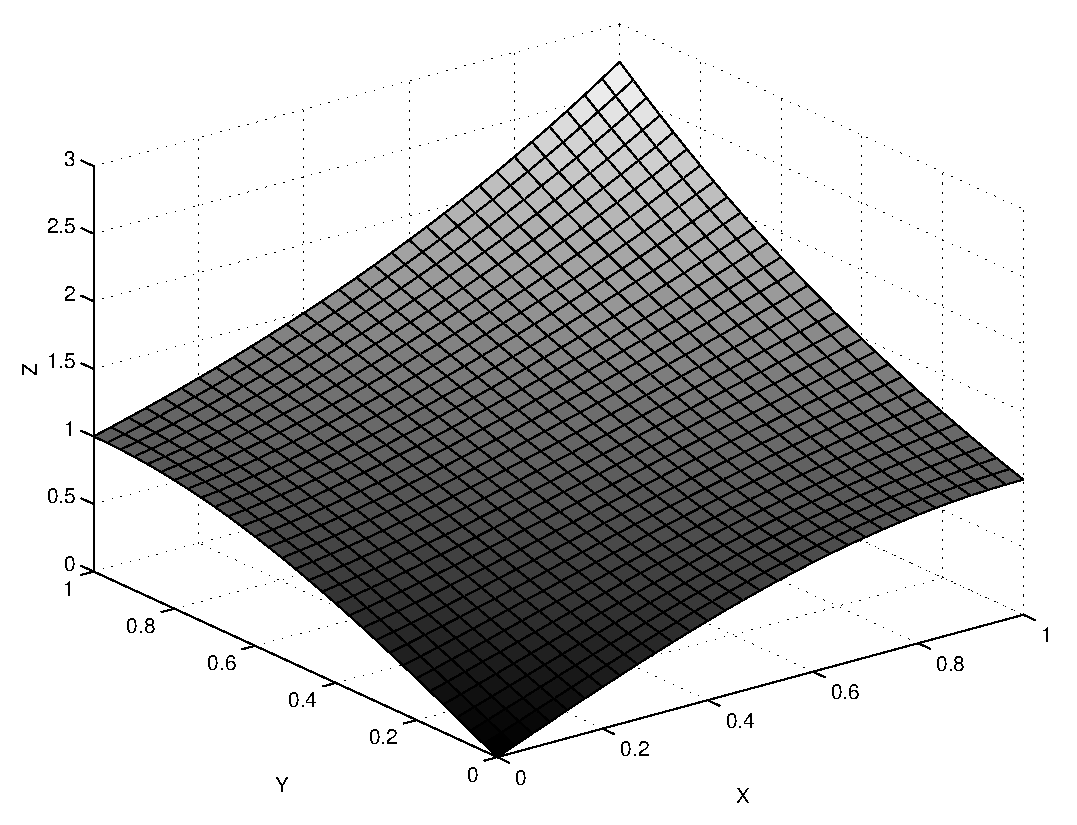
\includegraphics [scale = 0.3]{images/eq-poisson-modif.eps}
    \caption{Solution modified}
              \label{fig-eq-Poisson-modif}
    \end{center}
\end{minipage}
\end{figure}
 
 
\begin{rem}{(\upshape \textbf{Case of a quadratic functional}).} 
\index{Function!quadratic} If we consider an exact quadratic solution, for example the function $ u (x, \, y) = x^2 + y^2 $, which satisfies the Poisson equation:
\begin{equation*}
\pdd{u}{x} + \pdd{u}{y} = 4,
\end{equation*}
one notices that the error obtained during the resolution by a finite difference method is quasi-zero. This is explained by the fact that the approximation of the Laplacian by the equation \eqref{eq-poisson-discretise} is in fact exact for a polynomial of degree less than two (it is an interpolation formula of order of them).
\end{rem}
The exercise \oldref{exo-formulation-matrix-fish} takes up this method of resolution by explaining its operation by matrix decompositions.

% ------------------------------------------------- -----
% ------------------------------------------------- -----
% ------------------------------------------------- -----
% section - Product calculations                            
% ------------------------------------------------- -----
% ------------------------------------------------- -----
% ------------------------------------------------- -----
\section{Product calculations}
% \addcontentsline{toc}{section}{Product calculations}
\label{sect1-calculations-products} 
 
 
\index{Calculation!of products} Contrary to what one might think after all these applications dedicated to numerical calculation, the FFT algorithm has applications of a much more algebraic nature. It is mainly the convolution property that is used. This algorithm allowed significant advances for certain arithmetic calculations, for example for intensive calculations of large numbers (the search for decimals of $ \pi $ is the best example). We can read about this subject \cite{bailey-pi} which explains some instructive anecdotes.
% ------------------------------------------------- -----
% ------------------------------------------------- -----
% sub-section - Theoretical presentation                            
% ------------------------------------------------- -----
% ------------------------------------------------- -----
\subsection{Theoretical presentation}
\label{sect2-presentation-theoretical} 
 
 
Before describing methods using the FFT algorithm presented in paragraph \ref{sect2-present-algo-fft}, to calculate products, we can explain in a somewhat theoretical way the approach we are going to follow.
 
 
\index{Kernel} \index{Morphism} \index{Ideal} Consider, for $ (\xi_0, \ldots, \, \xi_{N-1}) \in \CC^N $, the evaluation morphism
\begin{equation*}
\Phi: \func{\CC [X]}{\CC^N}{P}{\left(P (\xi_0), \ldots, \, P (\xi_{N-1}) \right)} .
\end{equation*}
The kernel of this morphism is the ideal of $ \CC [X] $ generated by the polynomial $ \prod_{k = 0}^{N-1}{(X- \xi_k)} $. In the case where the points $ \xi_k $ are distinct, we obtain, by passing to the quotient, a linear isomorphism (since the two spaces have the same dimension $ N $)
\begin{equation*}
\wt{\Phi}: \left\{\begin{array}{ccc} \CC [X] / \prod_{k = 0}^{N-1}{(X- \xi_k)} & \xrightarrow{\simeq} & \CC^N \\\ol{P} & \mapsto & (\ol{P} (\xi_0), \ldots, \, \ol{P} (\xi_{N-1})) \end{array} \right. .
\end{equation*}
It is even evidently an isomorphism of algebra, if we endow $ \CC [X] $ with the product of the polynomials, and $ \CC^N $ with the product component by component.
 
 
Thanks to this evaluation morphism, and its inverse morphism (interpolation), we can draw the following diagram:
\begin{equation*}
\begin{CD} (P_0, \ldots, \, P_{N-1}), (Q_0, \ldots, \, Q_{N-1}) @> mult.polyn \hat{o} mes> \grdo (N^2)> (R_0, \ldots, \, R_{N-1}) \\@VV{\acute{e} valuation} V @A{interpolation} AA \\\begin{array}{l} (P (\xi_0), \ldots, \, P (\xi_{N-1})), \\(Q (\xi_0), \ldots, \, Q (\xi_{N-1})) \end{array} @>{one-time mult.}>{\grdo (N)}> (R (\xi_0), \ldots, \, R (\xi_{N-1})) \end{CD},
\end{equation*}
which suggests a new way to multiply two polynomials, passing \guill{downwards}, namely using the application
\begin{equation*}
\Psi: \func{\CC [X] \times \CC [X]}{\CC [X] / \prod{(X- \xi_k)}}{(P, \, Q)}{\Phi^{-1} (\Phi (\ol{P}) \cdot \Phi (\ol{Q}))},
\end{equation*}
where we denote by $ \ol{P} $ the class of $ P $ in the algebra $ \CC [X] / \prod{(X- \xi_k)} $. From what we have just said, this morphism therefore calculates the product of the two polynomials modulo the polynomial $ \prod{(X- \xi_k)} $. The natural questions are therefore the following. \begin{rs}
\item What choice to make for the points $ \{\xi_0, \ldots, \, \xi_{N-1} \} $ so that this new way of calculating a product is fast?
\item How to really get the product of the two polynomials, and not just the product modulo a certain polynomial?
\end{rs} In fact, we have already answered these two questions in chapter \oldref{chap-tfd}. It suffices to link the TFD to the evaluation of polynomials to reinvest the algorithms already constructed.
 
\begin{rem}
\index{Chinese!Lemma} The $ \wt{\Phi} $ isomorphism is in fact the canonical isomorphism given by the Chinese theorem:
\begin{equation*}
\CC [X] / \prod_{k = 0}^{N-1}{(X- \xi_k)} \xrightarrow{\simeq} \prod_{k = 0}^{N-1}{\CC [ X] / (X- \xi_k)} \simeq \CC^N.
\end{equation*}
Indeed, the $ X- \xi_k $ are prime among themselves (because the $ \xi_k $ are distinct), therefore the application of the theorem is licit, and the reduction modulo $ X- \xi_k $ sends a polynomial $ P $ on $ P (\xi_k) $.
\end{rem}
 
% ------------------------------------------------- -----
% ------------------------------------------------- -----
% sub-section - Multiplication of polynomials modulo $ \mbold{X^N-1} $                            
% ------------------------------------------------- -----
% ------------------------------------------------- -----
\subsection{Multiplication of polynomials modulo $ \mbold{X^N-1} $}
\label{sect2-multiplication-polynomials-modulo-xn-1} 
 
 
\index{Polynomial!multiplication} \index{Product!of polynomials} The aim of this paragraph is to present the Fourier transform as a transformation (in fact a morphism) on polynomials of fixed degrees. We can then use the algebraic properties of the discrete Fourier transform as well as the FFT algorithm to perform operations on polynomials very quickly. Behind these particularly efficient methods hides a more subtle problem than the simple use of the Fourier transform, since it is the question of the representation of polynomials. Indeed, the Fourier transform makes it possible to juggle between two types of representations, and thus to exploit the strengths of each.
 
 
The purpose of this approach being to reinvest the algorithms already presented in chapter \oldref{chap-tfd} (mainly FFT and fast convolution), we hasten to choose wisely the points of evaluation / interpolation $ \xi_k $, by l' occurrence, the $ N $ roots \ordin{N}{iès} of the unit, i.e. $ \xi_k = \omega_N^{- k} = e^{- \frac{2 \imath k \pi}{N}} $ for $ k = 0, \ldots, \, N-1 $. We see then that the morphism $ \wt{\Phi} $ is in fact the discrete Fourier transform. More precisely, we can rewrite it as follows:
\begin{equation*}
\wt{\Phi}: \left\{\begin{array}{ccc} \CC [X] / (X^N-1) & \xrightarrow{\simeq} & \CC^N \\\ol{P} & \mapsto & \wt{\Phi} (P) = \Ff(P_0, \ldots, \, P_{N-1}) \end{array} \right.,
\end{equation*}
where we denote by $ P_0, \ldots, \, P_{N-1} $ the coefficients of the polynomial $ \ol{P} $ (we have chosen the representative of degree less than $ N $). Of course, we used the identity $ \prod_{k = 0}^{N-1}{(X- \xi_k)} = X^N-1 $ here. We therefore notice that the computation of the discrete Fourier transform of $ P $ (as a vector of $ \CC^N $) is nothing other than the computation of the values that $ P $ takes in them. $ N $ roots \ordin{N}{ièmes} of the unit, and we find exactly the morphism $ \Phi $ of the previous paragraph.
 
 
The discrete Fourier transform thus makes it possible to juggle between two representations of polynomials of degree $ N-1 $ (in fact modulo $ X^N-1 $): \begin{rs}
\item \index{Representation!by coefficients} \textit{representation by coefficients}: this amounts to considering a polynomial as a vector of $ \CC^N $. Although very commonly used, this representation has a weak point: it is not at all suitable for calculating the product of two polynomials. While the sum of two polynomials $ P $ and $ Q $ of degree at most $ N $ is calculated in $ N $ operations (as shown by the equality $ (P + Q)_k = P_k + Q_k $), the product, calculated naively, requires $ N^2 $ operations.
\item \index{Representation!by values} \textit{representation by values}: we give ourselves the polynomial by the values it takes in $ N $ distinct points (here taken in a very particular way, the roots \ordin{N}{ith} of the unit). This representation is much more suited to the computation of the product, since it suffices to do the product of the values of each polynomial.
\end{rs} Take this literally: the FFT algorithm provides a quick and easy way to switch between representations.
 
 
To finish, let us recall the equation obtained for the computation of the product of two polynomials modulo $ X^N-1 $:
\begin{equation}
\label{eq-prod-cyclic-polynomial}
P * Q = \Ff^{-1} \left(\Ff(P) \cdot \Ff(Q) \right).
\end{equation}
\index{Convolution!circular} In this equation, we have confused vector and modulo polynomials $ X^N-1 $, and the product $ P * Q $ can also be seen as a product of circular convolution between two vectors. The operation performed can be graphically represented. The first two graphs in figure \figref{fig-convolution-polynomial} show the polynomials defined by $ P = 1 + 2X + X^3-X^4 + X^5 $ as well as $ Q = XX^2 + 2X^3 + 2X^5$. On the abscissa, we put the degrees of monomials $ 1, \ldots, \, X^{10} $. We therefore choose to work in $ \ZZ/11 \ZZ $. This makes sense, because the degree of the product $ P * Q $ is precisely $ 10 $. Thus, when we represent in the graph on the right the product of the two vectors, we find the graphical representation of the product $ P * Q $, since the reduction modulo $ X^{11} -1 $ did not have effect. \begin{figure}[ht]
    \begin{center}
    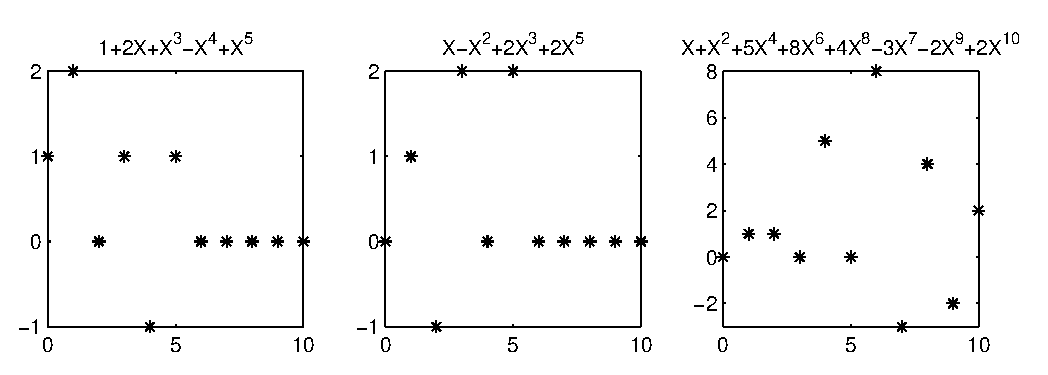
\includegraphics[scale=0.7]{images/convolution-polynome.eps}
    \end{center}
    \caption{Graphical representation of the product of polynomials by convolution}
              \label{fig-convolution-polynomial}
\end{figure}
 
 
\begin{rem}{(\upshape \textbf{Lagrange interpolation}).} 
Algorithms make it possible to calculate the interpolation polynomials in the case where the points $ \xi_k $ are not necessarily roots of the unit. There is of course the result of \textit{Lagrange}, which gives an explicit basis of $ \CC_{N-1}[X] $ (space of polynomials of degree at most $ N-1 $) in which the computation is done simply. Indeed, if we look for the polynomial $ P $ which takes the values $ y_i $ at the points $ x_i $, for $ i = 0, \ldots, \, N-1 $, then $ P = \sum_{i = 0}^{N-1}{y_i P_i} $, where $ P_i $ is the \ordin{i}{rd} \textit{Lagrange polynomial} associated with the points $ \{x_i \}_{i = 0}^{N-1} $:
\begin{equation*}
P_i \eqdef \frac{\prod_{j = 0}^{N-1} (X-x_j)}{\prod_{j \neq i} (x_i-x_j)}.
\end{equation*}
\index{Difference!divided} \index{Lagrange!polynomial} However, the numerical computation of the interpolation polynomial in the base of $ \{P_i \}_{i = 0}^N $ is not used in practice, because it leads to an accumulation of numerical errors. We prefer to use the \textit{divided differences} technique, which is explained for example in \cite{demailly}.
\end{rem}
 
% ------------------------------------------------- -----
% ------------------------------------------------- -----
% sub-section - Multiplication of polynomials                            
% ------------------------------------------------- -----
% ------------------------------------------------- -----
\subsection{Multiplication of polynomials}
\label{sect2-multiplication-polynomials} 
 
 
The difficulty with which we are faced when calculating the product of two polynomials $ P $ and $ Q $ (of degree $ N-1 $) by the method presented above is that a priori, the product $ PQ $ is a polynomial of degree $ 2N-2 $. This polynomial will therefore be reduced modulo $ X^N-1 $, which often has a more than undesirable effect ... More precisely, the coefficients of the product are given by the equation
\begin{equation}
\label{eq-product-polynomials}
\forall n \in \{0, \ldots, \, 2 N - 1 \}, \quad (PQ)_n = \sum_{k = 0}^{n}{P_k Q_{n - k}}.
\end{equation}
\index{Convolution!acyclic} It is in fact an acyclic convolution product (to be compared to the cyclic product of the equation \eqref{eq-prod-cyclic-polynomial}), and we will be able to use the technique already presented in the Section~\ref{sect1-convolution-acyclic}, to calculate it.
 
 
\index{Convolution!circular} This approach (adding zeros at the end of the vector to make the product cyclic) is very intuitive, since it consists in considering the two polynomials as polynomials of degree $ 2N-1 $ (by adding zero coefficients). We can then apply the approach presented in the previous paragraph (ie use a cyclic convolution product, or if you prefer, calculate the product modulo $ X^{2N} -1 $). Fortunately, this does not change the result, since the polynomial $ PQ $ is not affected by the reduction modulo $ X^{2N} -1 $. In a more theoretical way, this amounts to using the bijectivity of the application
\begin{equation*}
\func{\CC_{2N-1}[X]}{\CC [X] / (X^{2N} - 1)}{P}{P \mod{X^{2N} - 1}},
\end{equation*}
where we denote by $ \CC_{2N-1}[X] $ the space of polynomials of degree less than or equal to $ 2N-1 $.
% ------------------------------------------------- -----
% ------------------------------------------------- -----
% sub-section - Multiplication of large integers                            
% ------------------------------------------------- -----
% ------------------------------------------------- -----
\subsection{Multiplication of large integers}
\label{sect2-multiplication-integers} 
 
 
\index{Integer!multiplication} \index{Calculation!of products of integers} \index{Product!of integers} We denote by $ (a_0, \ldots, \, a_{N-1}) $ the base representation $ b $ of a large integer $ a $, that is
\begin{equation*}
a = a_0 + a_0 b + \cdots + a_{N-1} b^{N-1}.
\end{equation*}
\index{Matlab@\Matlab{}} We notice that the multiplication of two integers $ a $ and $ a'$ is similar to the calculation of a product of polynomials, with one exception: the integers $ a_k $ and $ a'_k $, for $ k = 0, \ldots, \, N-1 $, must belong to the set $ \{0, \ldots, \, b-1 \} $. If we want to quickly compute the multiplication of two large integers, we can therefore use the polynomial product technique that we have just exposed in the previous paragraph, followed by a \guill{carry propagation} phase. \Matlab{} programs allowing to achieve all this are gathered in the paragraph \annexeref{sect1-listing-mult-integers}.
 
 
This approach nevertheless suffers from some weak points, mainly related to the use of floating point calculations (for the classic FFT algorithm), which are subject to rounding errors (while integer calculations are both faster and free of errors). This problem will be solved in chapter \ref{chap-extension-finite-field-values}, thanks to the introduction of the Fourier transform on finite fields and rings.

% ------------------------------------------------- -----
% ------------------------------------------------- -----
% ------------------------------------------------- -----
% section - Exercises                            
% ------------------------------------------------- -----
% ------------------------------------------------- -----
% ------------------------------------------------- -----
\section{Exercises}
% \addcontentsline{toc}{section}{Exercises}
\label{sect1-chap3-exercises} 
 
 
 
\begin{exo}[Compactly supported transform]
\label{exo-transforme-sup-comp}
 
\index{Support!compact} We have to prove the proposition \ref{prop-trans-fourier-support-compact}. Let $ f $ be a function such that $ \Supp (\wh{f}) \subset [-A, \, A] $. Explain why $ f $ is of class $ \Cc^{\infty} $, and calculate its successive derivatives $ f^{(n)} (t_0) $, for $ t_0 \in \RR $, as an integral between $ -A $ and $ A $. Using a limited expansion of $ t \mapsto e^{\imath t} $ in $ t_0 $, deduce an expansion of $ f $. Deduce that $ f \neq 0 $ cannot vanish over a whole nonempty interval.
\end{exo}
 
 
\begin{exo}[Solving the heat equation by finite differences]
\label{exo-resol-eq-heat-diff-finies}
 
\index{Equation!of heat} \index{Difference!finite} We want to solve in an approximate way the equation of heat on the circle, whose formulation we recall, for $ \kappa = 1 $:
\begin{equation}
\label{eq-heat-exo}
\left\{\begin{array}{l} \forall (t, \, x) \in \RR_*^{+} \times S^1, \quad \pd{u}{t} = \pdd{u}{x} \\\forall x \in S^1, \quad u (0, \, x) = f(x) \end{array} \right. ,
\end{equation}
where the sought solution $ u $ is assumed to be sufficiently regular over $ \RR_*^{+} \times S^1 $, and continues over $ \RR^{+} \times S^1 $. To do this, we consider a discretization of step $ d = \frac{1}{N} $ in space, and of step $ h $ in time. This leads us to consider the vectors $ u^n \in \RR^N $, for $ n \geq 0 $, supposed to approximate the function $ u $:
\begin{equation*}
\forall n \geq 0, \; \forall k \in \{0, \ldots, \, N-1 \}, \quad u^n [k] \approx u (nh, \, kd).
\end{equation*}
\begin{enumerate}
\item Show that we can, following a discretization of the equation \eqref{eq-heat-exo}, consider the difference equation
\begin{equation*}
u^{n + 1}[k] - u^n [k] = s \left(u^n [k + 1] + u^n [k-1] - 2 u^n [k] \right) ,
\end{equation*}
for $ n \geq 0 $ and $ k = 1, \ldots, \, N-1 $. We have noted $ s \eqdef \frac{h}{d^2} $, and by convention, we define $ u^n [-1] \eqdef u^n [N-1] $ and $ u^n [ N] \eqdef u^n [0] $.
\item \index{Matlab@\Matlab{}} Show that this explicit scheme can be written in the form of a convolution. Is it advantageous to compute $ u^n $ by iterated convolutions using the FFT algorithm? Propose a \Matlab{} implementation of the chosen algorithm.
\item We say that the chosen numerical scheme is stable if, for any $ u_0 $ such that $ \norm{u_0}_{\infty} \leq 1 $, then the approximate solution $ u^n $ remains bounded whatever $ n $. Give, using the discrete Fourier transform, a necessary and sufficient condition for the scheme we have just built to be stable.
\item \index{Schema!explicit} \index{Schema!implicit} \index{Stability} We now want to consider non-explicit schemas, that is to say such that $ u^{n + 1} $ is not not given directly in terms of $ u^{n} $. We consider the scheme
\begin{equation*}
u^{n + 1} - u^{n} = A * \left(\theta u^{n + 1} + (1- \theta) u^{n} \right),
\end{equation*}
where $ \theta $ is a varying parameter in $ [0, \, 1] $, and $ A $ is the vector such that $ A [0] = - 2s $, $ A [1] = A [-1] = s $, and all other entries are zero. In particular, we notice that for $ \theta = 0 $ we find the explicit scheme already constructed, and that for $ \theta = 1 $, we obtain an implicit scheme. Explain how we can solve this equation using the Fourier transform. Then study the problem of the stability of the diagram obtained.
\item Resume the previous questions in the case of the heat equation in dimension 2, that is to say on $ \RR^+ \times S^1 \times S^1 $. In particular, we will propose an implementation of the implicit algorithms using two-dimensional FFT calculations.
\end{enumerate} \index{Image} Figure \figref{fig-eq-heat-finite-diff} shows the solution of the 2D heat equation by different schemes. Horizontally, each image represents a step of the algorithm. The first line corresponds to $ \theta = 0 $, and with an image of size $ 256 \times 256 $, we verify that we must take $ h $ of the order of $ 10^{- 6} $ so that the diagram either stable (this condition is of course not verified in the figure, where we have $ h = 0.0002 $). The second line corresponds to $ \theta = 0.5 $, but with such a large step, we can see that some instabilities appear. Finally, the last line corresponds to $ \theta = 1 $, and the scheme is very stable. 

\begin{figure}[ht]
    \begin{center}
    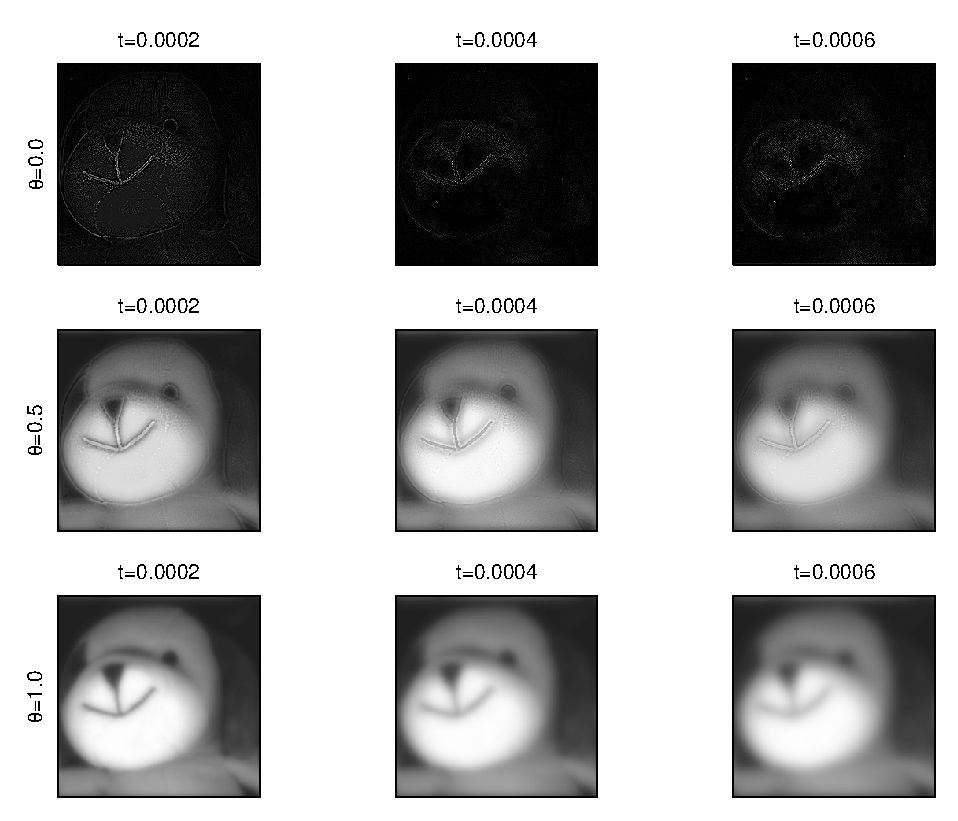
\includegraphics[scale=0.7]{images/eq-chaleur-diff-finie.eps}
    \end{center}
    \caption{Solving the heat equation by finite differences}
              \label{fig-eq-heat-finite-diff}
\end{figure}
\end{exo}
 
 
\begin{exo}[Uniqueness for the heat equation]
\label{exo-unicite-eq-heat}
 
\index{Equation!of heat} This proof is taken from the book of \nompropre{Dym} and \nompropre{McKean}{\upshape \cite{dym}}. We consider the heat equation on the circle \eqref{eq-heat-exo}. We want to show that under the $ f $ continuous hypothesis, the equation \eqref{eq-solution-heat-equation} does indeed define a solution of the equation, and that it is in fact the only one. \begin{enumerate}
\item Show that for $ t> 0 $, the solution $ u $ can be written as a convolution:
\begin{equation*}
u (t, \, x) = p_t * f(x) \quad \text{with} \quad p_t (x) \eqdef \sum_{n \in \ZZ}{e^{- 2 \pi^2n^2 t} e_n (x)}.
\end{equation*}
 
\item In the case where $ f \in \Cc^2 (S^1) $, show that we have $ \norm{u (t, \, \cdot) - f}_{\infty} \tv{t \to 0} $ 0.
\item We want to show that if $ f \geq 0 $, then $ u \geq 0 $. We consider the function $ v $ defined $ v (t, \, x) = e^{\beta t} u (t, \, x) $, for a certain parameter $ \beta $. Show that if we assume that $ u (t_0, \, x_0) <0 $, the function $ v $ reaches its minimum $ \alpha <0 $ on $ [0, \, t_0] \times S^1 $ for a some time $ t_1> 0 $ and a position $ x_1 $. Show while we have
\begin{equation*}
0 \geq \pd{v}{t} (t_1, \, x_1) = \alpha \beta + \frac{1}{2} \pdd{u}{x} (t_1, \, x_1) \geq \alpha \beta
\end{equation*}
Deduce a contradiction by taking $ \beta <0 $.
\item \index{Principle!of the maximum} Using the convolution product that defines $ u $, deduce that $ p_t $ is positive. Deduce the \textit{maximum principle} for the heat equation:
\begin{equation*}
\forall t> 0, \quad \norm{u (t, \, \cdot)}_{\infty} \leq \norm{f}_{\infty}.
\end{equation*}
Show that this ensures the uniqueness of the solution of the heat equation.
\item Using a sequence of functions $ f_n \in \Cc^2 (S^1) $ which converges uniformly to $ f $, deduce that in the case where $ f $ is simply continuous, we still have the convergence $ \norm{u (t, \, \cdot) - f}_{\infty} \tv{t \to 0} 0 $.
\end{enumerate}
\end{exo}
 
 
\begin{exo}[3D electric potential]
\label{exo-potential-electric-3d}
 
\index{Electric potential} We want to generalize the algorithm for solving the Poisson equation described in paragraph \ref{sect2-resol-eq-Poisson} for three-dimensional problems. For example, we want to determine an electric potential $ u $ which satisfies the Poisson equation:
\begin{equation*}
\forall (x, \, y, \, z) \in [0, \, 1] \times [0, \, 1] \times [0, \, 1], \quad \Delta u (x, \, y, \, z) \eqdef \pdd{u}{x} + \pdd{u}{y} + \pdd{u}{z} = f(x, \, y, \, z),
\end{equation*}
with boundary conditions as well as a user-specified function $ f $. It will of course be necessary to use a three-dimensional Fourier transform, and to think about making the encountered 3D arrays odd. To represent the solution, we can draw equipotential surfaces, i.e. the surfaces of equation $ f(x, \, y, \, z) = \lambda $ for certain values of the parameter $ \lambda $ .
\end{exo}
 
 
\begin{exo}[Matrix formulation for the Poisson equation]
\label{exo-formulation-matrix-fish}
 
This exercise, which offers a more computational explanation of the algorithm for solving the Poisson equation, is partly inspired by the article by \nompropre{Swarztrauber} and \nompropre{Sweet}{\upshape \cite{swarztrauber}}. We take the notations of paragraph \ref{sect2-resol-eq-Poisson}, and we consider in particular a square matrix $ U $ of size $ N-1 $ (the indices varying from $ 1 $ to $ N-1 $) which is the solution of the finite difference equation \eqref{eq-poisson-discretise} inside the square $ [0, \, 1] \times [0, \, 1] $ (that is say without the boundary terms). \begin{enumerate}
\item Without taking into account the boundary terms, show that we can write the difference equation in the form
\begin{equation*}
T_{N-1} U + U T_{N-1} = F,
\end{equation*}
where $ T_{N-1} $ is the matrix of size $ N-1 $ with $ -2 / h^2 $ on the diagonal and $ 1 / h^2 $ on the sub-diagonal and the over-diagonal.
\item Since the value of the solution on the edges is assumed to be known, use the same approach as that employed in paragraph \ref{sect2-resol-eq-Poisson} to obtain a modified equation of the type
\begin{equation}
\label{eqn-exo-matrix-formulation-1}
T_{N-1} \wt{U} + \wt{U} T_{N-1} = \wt{F}.
\end{equation}
 
\item Show that the eigenvectors of $ T_{N-1} $ are the
\begin{equation*}
V_j \eqdef \left\{\sin \left(\frac{ij \pi}{N} \right) \right\}_{i = 1}^{N-1}.
\end{equation*}
Determine the associated eigenvalues. We denote by $ V $ the base change matrix, which means that its columns are the $ V_j $, and $ D $ the diagonal matrix whose inputs are the calculated eigenvalues. By noting $ U_0 \eqdef V^{-1} \wt{U} V $ and $ \wt{F}_0 = V^{-1} \wt{F} V $, deduce that $ U_0 $ satisfies l'equation
\begin{equation*}
D U_0 + U_0 D = \wt{F}_0.
\end{equation*}
Solve this equation.
\item \index{Transform!into sine} Show that the matrix $ V $ is in fact orthogonal, and that the computation of $ V x $, where $ X $ is a matrix of size $ N-1 $, is equivalent to a calculation of \textit{sine transform} (that is to say the imaginary part of a certain discrete Fourier transform). Deduce that the computation of $ \wt{U} = V U_0 V^{-1} $ is in fact equivalent to the computation of a two-dimensional sine transform (i.e. a transform on the lines followed by'a transform on the columns of a matrix).
\item Explain how we can calculate sine transforms (unidimensional then in 2D) thanks to a DFT of double size. How to calculate the inverse transform? Finally, make the connection between the matrix approach proposed in this exercise and the computation of convolution which supported the algorithm proposed in Paragraph~\ref{sect2-resol-eq-Poisson}.
\end{enumerate}
\end{exo}
 
 
\begin{exo}[Image smoothing]
\label{exo-lissage-image}
 
\index{Image smoothing} \index{Gaussian} \index{Image} \index{Filter!2D} Write a program that smooths a 2D image in grayscale, as shown in the figure \figref{fig-filter-2d}. We can use a Gaussian transfer function, and adapt the parameters to the size of the image.
\end{exo}
 
 
\begin{exo}[Correlation and image detection]
\label{exo-correlation-2d}
 
\index{Image} This exercise is inspired by an article by \nompropre{Lewis}{\upshape \cite{lewis}}, which brings up to date the use of correlation for image detection. Let $ f \in \RR^{N \times N} $ be an image of size $ N $, and $ g \in \RR^{P \times P} $ another image, typically much smaller in size than that of $ f $. The question is to determine if the image $ g $ is a subimage of $ f $, and if so, to locate its location. For this purpose, we define the distance between $ f $ and $ g $
\begin{equation*}
\forall (u, \, v) \in \{0, \ldots, \, N-1 \}^2, \; d (f, \, g) [u, \, v]^2 \eqdef \sum_{(x, \, y) \in D (u, \, v)}{\left(f(x, \, y) - g (xu, \, yv) \right)^2},
\end{equation*}
where $ D (u, \, v) $ denotes the subset of $ \{0, \ldots, \, N-1 \}^2 $ formed by the pairs $ (x, \, y) $ such that $ (xu, \, yv) \in \{0, \ldots, \, P-1 \}^2 $. \begin{enumerate}
\item \index{Correlation} \label{notation-55} What is the intuitive meaning of $ d (f, \, g) $? In what circumstance is $ d (f, \, g) $ close to zero? In the event that the quantity
\begin{equation*}
P_{u, v} (f) = \sum_{(x, \, y) \in D (u, \, v)}{f(x, \, y)^2}
\end{equation*}
is almost constant, showing that finding the points where $ d (f, \, g) $ is small amounts to maximizing the \textit{correlation} between $ f $ and $ g $
\begin{equation*}
\Corr (f, \, g) [u, v] \eqdef \sum_{(x, \, y) \in D (u, \, v)}{f(x, \, y) \, g ( xu, \, yv)}.
\end{equation*}
 
\item \index{Acyclic!convolution} Show that $ \Corr (f, \, g) $ can be written as an acyclic convolution product. Deduce that we can calculate this correlation quickly using the FFT algorithm.
\item \index{Correlation!normalized} \label{notation-56} We want to correct the defect we introduced by supposing that $ P_{u, v} (f) $ is almost constant. We denote by $ \wt{f}_{u, v} $ the average of $ f $ over $ D (u, \, v) $, and $ \wt{g} $ the average of $ g $. We then define the \textit{normalized correlation}
\begin{equation*}
\ol{\Corr} (f, \, g) [u, \, v] \eqdef \frac{\sum_{(x, \, y)}{(f(x, \, y) - \wt{f}_{u, v}) (g (xu, \, yv) - \wt{g})}}{\left\{\sum_{(x, \, y)}{(f(x, \, y) - \wt{f}_{u, v})^2} \, \sum_{(x, \, y)}{(g (x, \, y) - \wt{g})^2} \right\}^{1/2}},
\end{equation*}
where the sums relate to $ (x, \, y) \in D (u, \, v) $. Explain how this quantity actually provides a correction. Do we still have a fast FFT calculation algorithm?
\item \index{Sliding sum} Show that the numerator of $ \ol{\Corr} (f, \, g) $ is written as a convolution. We denote, for $ k = 1, \, 2 $, the \guill{sliding sums}
\begin{equation*}
\forall (u, \, v) \in \{0, \ldots, \, N-1 \}^2, \quad s_k (u, \, v) \eqdef \sum_{(x, \, y) \in D (u, \, v)}{f [x, \, y]^k},
\end{equation*}
with by convention $ s_k (u, \, v) = 0 $ for $ u \geq N $ or $ v \geq N $. Show that $ s_k $ satisfies the recurrence equation
\begin{align*}
s_k (u, \, v) & = s_k (u + 1, \, v) + s_k (u, \, v + 1) - s_k (u + 1, \, v + 1) \\
& + f(u, \, v) + f(u + P, \, v + P) - f(u, \, v + P) - f(u + P, \, v).
\end{align*}
\index{Complexity} Deduce a fast computation algorithm of $ s_k $ (evaluate its complexity), then of $ \ol{\Corr} (f, \, g) $.
\end{enumerate} Figure \figref{fig-correlation-2d} shows an example of application of this method. We can clearly see that the normalized correlation (image (d)) has a much sharper maximum than the non-normalized correlation (image (c)). We can note that{\upshape \cite{lewis}} proposes a fast calculation algorithm which was used among other things to perform the readjustments in the movie \textit{Forest Gump} (1994). \begin{figure}[ht]
    \begin{center}
    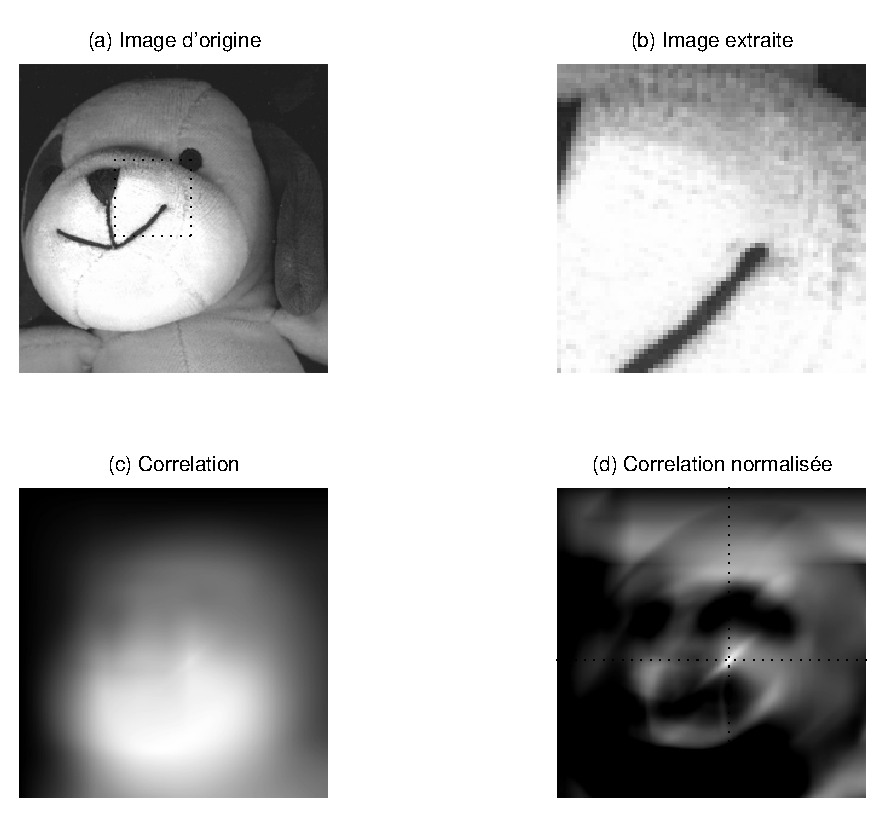
\includegraphics [scale = 0.7]{images/correlation-2d.eps}
    \end{center}
    \caption{Correlation between two images}
              \label{fig-correlation-2d}
\end{figure}
\end{exo}
 
 
\begin{exo}[Rotation by FFT]
\label{exo-fft-rotation}
 
Let $ f \in \CC^{N \times N} $ be a two-dimensional signal. We define, for $ v = (v_1, \, v_2) \in \RR^2 $ and $ \lambda \in \RR $,
\begin{equation*}
T_v (f) [k, \, l] = f [k-v_1, \, l-v_2], \quad S_\lambda^{(x)} (f) [k, \, l] = f [k - \lambda l, \, l], \quad S_\lambda^{(y)} (f) [k, \, l] = f [k, \, l- \lambda k].
\end{equation*}
\index{Rotation} \begin{enumerate}
\item \index{Translation} \index{Image} \index{Signal} Express $ \Ff(T_v (f)) $ in terms of $ \Ff(f) $. Deduce a fast algorithm to carry out any translation of an image. By translating each row (resp. Each column) by $ f $, write a fast algorithm to calculate $ S_\lambda^{(x)} (f) $ (respectively $ S_\lambda^{(y)} (f) $).
\item Show that a rotation of angle $ \theta $ around the origin can be written in the form
\begin{equation*}
\begin{pmatrix} \cos (\theta) & - \sin (\theta) \sin (\theta) & \sin (\theta) \end{pmatrix} = \begin{pmatrix} 1 & \lambda_1 \\0 & 1 \end{pmatrix} \begin{pmatrix} 1 & 0 \\\lambda_2 & 1 \end{pmatrix} \begin{pmatrix} \\1 & \lambda_3 0 & 1 \end{pmatrix}.
\end{equation*}
With the previous question, deduce a fast algorithm for rotating an image $ f \in \CC^{N \times N} $ around the origin.
\item What are the advantages and disadvantages of this algorithm? How to solve them? How to rotate an image around its center?
\end{enumerate} The figure \figref{fig-fft-rotation} shows several rotations of an image around its center. \begin{figure}[ht] 
    \begin{center}
    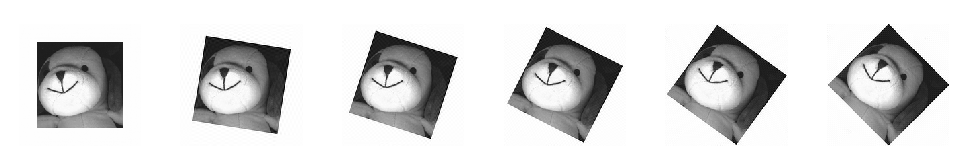
\includegraphics [scale = 0.9]{images/fft-rotation.eps}
    \end{center}
    \caption{Rotation of an image by FFT}
              \label{fig-fft-rotation}
\end{figure}
\end{exo}
 
 
\begin{exo}[Low pass filter]
\label{exo-creation-low-pass-filter}
 
\index{Filter!low pass} We want to create a low pass convolution filter. \begin{enumerate}
\item Write a \Matlab{} program which builds a vector $ f $, of size $ N $, such that the filter $ \Phi^f $ keeps the low frequencies $ N / 2 $, and removes the $ N / 2 $ high frequencies.
\item \index{Impulse!response} \index{Frequency!response} Represent with great precision the continuous Fourier transform of the impulse response $ f $ (in other words the frequency response of the filter). What do we see?
\item Considering a less brutal cut in the conserved / rejected frequencies, go back to the previous questions and comment on the results. In particular, imagine a family of filters $ f_{\epsilon} $, $ \epsilon \in [0, \, 1] $, with a sharp cutoff for $ \epsilon = 0 $ and soft for $ \epsilon = 1 $ .
\end{enumerate} Figure \figref{fig-low-pass-filter} shows three different filters, with increasingly softer cuts. We can also see the discrete filter transforms, and their continuous Fourier transforms. \begin{figure}[ht]
    \begin{center}
    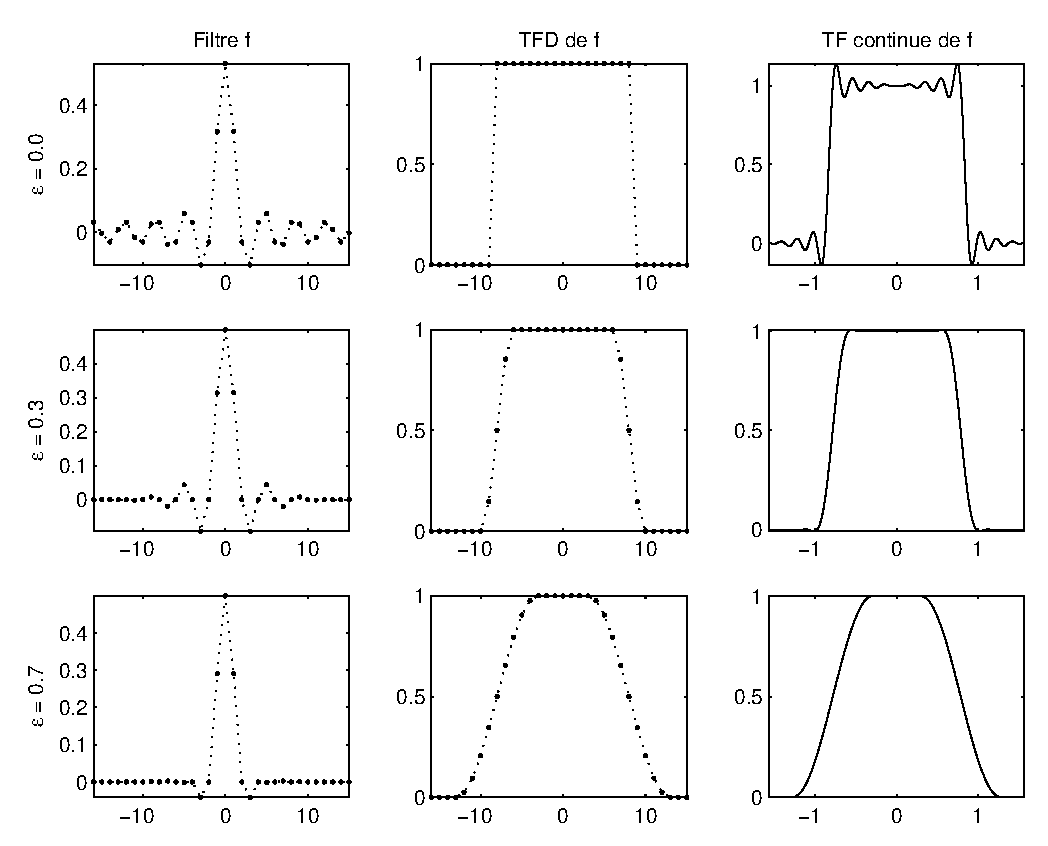
\includegraphics[scale=0.7]{images/filtre-passe-bas.eps}
    \end{center}
    \caption{Lowpass filters for different values of $ \epsilon $}
              \label{fig-low-pass-filter}
\end{figure}
\end{exo}
 
 
\begin{exo}[Integer iterations]
\label{exo-iterations-integers}
 
\index{Integer!iteration} We consider the following experiment: we have $ n $ children in a circle, and we give them each an even, arbitrary number of candies. The game consists in having each child give his neighbor on the right half of his candy, and to iterate the process. \begin{enumerate}
\item We arrange for the children to have an even number of candies each time they share. For this, an external person distributes, after each iteration, a candy to each child with an odd number of candies. Show that after a finite number of iterations, all the children have the same number of candies.
\item If we allow fractional parts of candies, show how we can translate this experiment into a convolution calculus. Deduce that after a potentially infinite number of iterations, all children have the same number of candies.
\item Study the first two questions for different sharing rules. For example, what if each child gives half of their candy to their neighbor on the left, and the other half to their neighbor on the right?
\end{enumerate}
\end{exo}
 
 
\begin{exo}[Karatsuba algorithm]
\label{exo-algo-karatsuba}
 
\index{Algorithm!of Karatsuba} \index{Karatsuba@\nompropreindex{Karatsuba}} \index{Calculation!of products of polynomials} \index{Divide to rule} We are going to explain the construction of a recursive polynomial multiplication algorithm . It uses a technique called \textit{divide and reign}, often used in algorithms, see for example the book of \nompropre{Cormen}{\upshape \cite{cormen}} for other examples. We consider two polynomials $ P $ and $ Q $ of degree $ n $ over a field $ K $. We denote by $ k \eqdef \lfloor (n + 1) / 2 \rfloor $. \begin{enumerate}
\item We write the polynomials $ P $ and $ Q $ in the form
\begin{equation*}
P (X) = P_0 (X) + X^k P_1 (X) \quad \text{and} \quad Q (X) = Q_0 (X) + X^k Q_1 (X),
\end{equation*}
where the polynomials $ P_0, Q_0 $ are of degree less than $ k $, and the polynomials $ P_1, Q_1 $ are of degrees less than $ k $ or $ k + 1 $, depending on the parity of $ n $. Show that the product $ P (X) Q (X) $ can be in the form
\begin{equation*}
P (X) Q (X) = R_0 (X) + X^k R_1 (X) + X^{2 k} R_2 (X).
\end{equation*}
Specify the value of the polynomials involved in this equality.
\item Show that the polynomial $ R_1 $ can be calculated using only one multiplication, but on the other hand 4 additions.
\item \index{Complexity} Implement a recursive algorithm using the decomposition we have just performed at each step. \\Prove that the complexity of this algorithm is $ \grdo (n^{\log_2 (3)}) $. For which values of $ n $ this algorithm is preferable to the algorithm using the FFT described in paragraph \ref{sect2-multiplication-polynomials}?
\end{enumerate}
\end{exo}
 
 
\begin{exo}[Spline and filtering]
\label{exo-spline-filtering}
 
\index{Spline} \index{B-spline} \index{Interpolation!direct} \index{Interpolation!indirect} This exercise requires some knowledge of Fourier series. If $ \{f [k] \}_{k \in \NN} $ is a sequence of $ \ell^2 (\ZZ) $, we define its Fourier transform by
\begin{equation*}
\forall x \in \RR, \quad \wh{f} (x) \eqdef \sum_{k \in \ZZ}{f [k] e^{- \imath kx}}.
\end{equation*}
It is a $ 2 \pi $ -periodic function, which we can assimilate to a function of $ L^2 (\RR / 2 \pi \ZZ) $. \\Let $ u: \RR \rightarrow \RR $ a continuous function which decreases fast enough to $ \pm \infty $. We assume that we actually know sampled values of $ u $, denoted by $ u_d [k] \eqdef u (k) $, for $ k \in \ZZ $. We want to interpolate these values in one of the two following forms:
\begin{align}
\label{eq-direct-interpolation}
v (x) \eqdef & \sum_{k \in \ZZ}{u_d [k] \varphi (xk)} \\
\label{eq-indirect-interpolation}
v (x) \eqdef & \sum_{k \in \ZZ}{a [k] \psi (xk)},
\end{align}
\index{Support} the functions $ \varphi $ and $ \psi $ being given in advance, with a little support. We assume of course that the interpolation is exact, ie $ \forall k \in \ZZ, \; v (k) = u (k) $. The sequence $ a [k] $, $ k \in \ZZ $, is unknown, and we will have to determine it. The \eqref{eq-direct-interpolation} interpolation scheme corresponds to direct interpolation, while \eqref{eq-indirect-interpolation} corresponds to indirect interpolation. \begin{enumerate}
\item We denote by $ \psi_d [k] \eqdef \psi (k) $ the sampled sequence of $ \psi $. We suppose that
\begin{equation*}
\forall \xi \in \RR, \quad \wh{\psi_d} (\xi) \neq 0.
\end{equation*}
Show then that the indirect interpolation problem admits a solution $ c $ uni \-que, given by the relation
\begin{equation*}
\forall \xi \in \RR, \quad \wh{c} (\xi) = \frac{\wh{u} (\xi)}{\wh{\psi_d} (\xi)}.
\end{equation*}
How can we reduce this interpolation to a direct interpolation? What problem are we encountering?
\item \label{notation-57} We define the B-spline function of order $ n $, denoted $ \beta^n $ by
\begin{equation*}
\beta^0 = 1_{[- \frac{1}{2}, \, \frac{1}{2}]} \quad \text{and} \quad \forall n> 0, \quad \beta^n = \beta^0 * \beta^{n-1}.
\end{equation*}
\index{Support} What is the support for $ \beta^n $? Do these functions allow you to define a direct interpolation scheme? Indirect? The figure \figref{fig-box-spline} shows the first 4 spline functions $ \beta^n $. 

\begin{figure}[ht]
    \begin{center}
    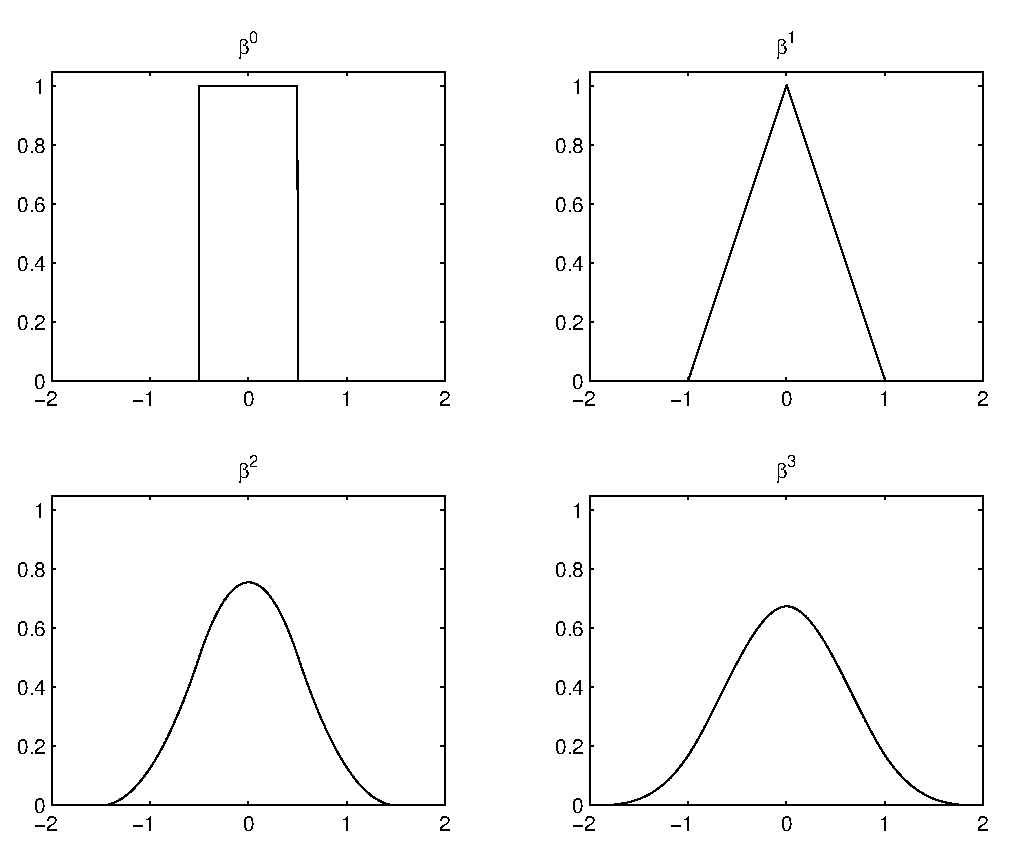
\includegraphics [scale = 0.5]{images/box-spline}
    \end{center}
    \caption{Basic spline functions}
              \label{fig-box-spline}
\end{figure}
 
\item Calculate the value of $ \wh{\beta^n} $ (continuous Fourier transform). We denote by $ \beta^n_d $ the sequence sampled from $ \beta^n $. Calculate the value of $ \wh{\beta^n_d} $ (Fourier series), and show that this function does not vanish (we will have to distinguish according to the parity of $ n $).
\item Deduce an expression of the function $ \beta^n_{card} $ which allows to perform an indirect interpolation from spline functions. What is its support? Show that we have the following convergence, in $ L^2 (\RR) $:
\begin{equation*}
\beta^n_{card} \tv{n \to \pinf} \sinc, \quad \text{where} \quad \sinc (x) \eqdef \frac{\sin (\pi x)}{\pi x}.
\end{equation*}
When $ n \rightarrow \infty $, what kind of interpolation do we perform? The figure \figref{fig-comparison-spline-sinc} shows a comparison between the cardinal functions corresponding to the spline interpolation of degree 3 (i.e. $ \beta^3_{\text{card}} $ ) and Shannon interpolation (i.e. $ \sinc $). We see that the spline function has a lot less \guill{bounces}. 

\begin{figure}[ht]
    \begin{center}
    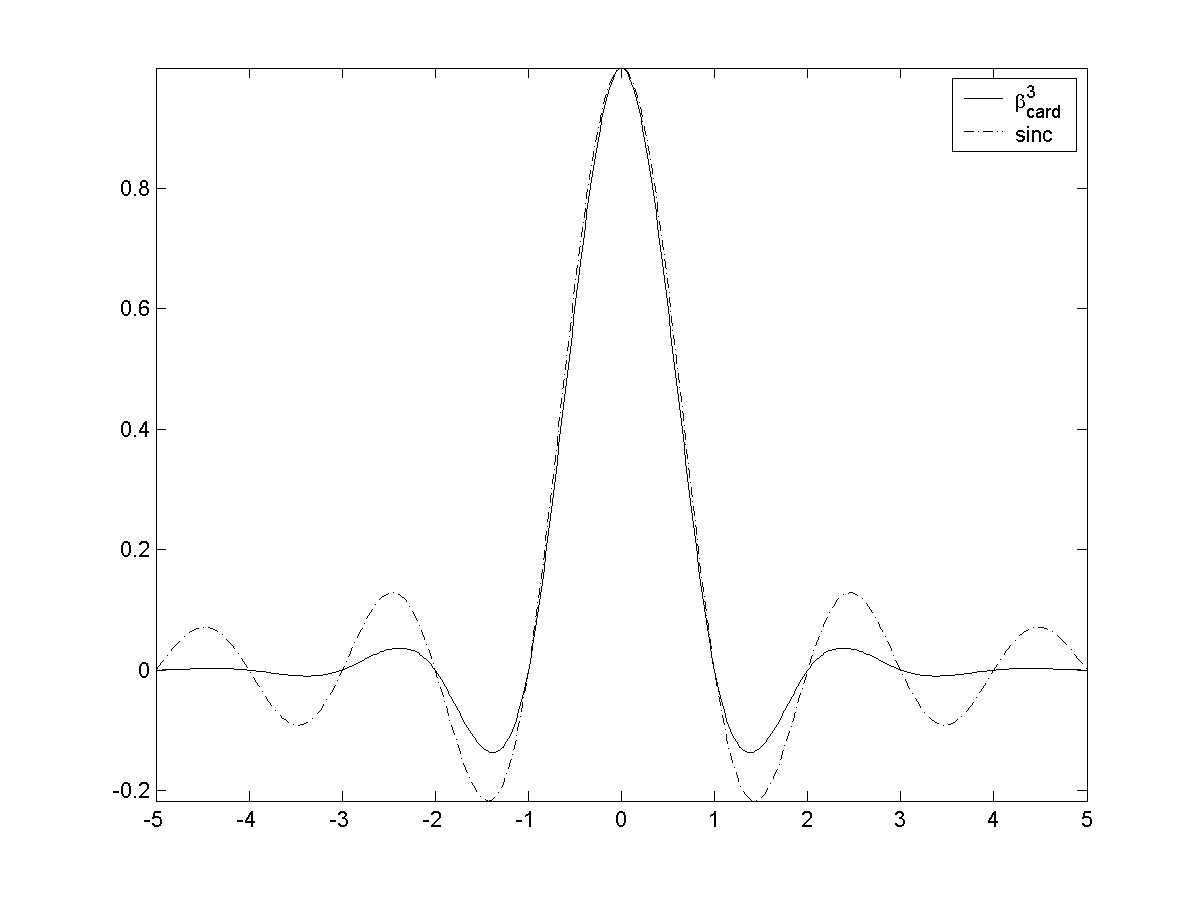
\includegraphics[scale=0.4]{images/comparaison-spline-sinc}
    \end{center}
    \caption{Comparison between spline and cardinal sine}
              \label{fig-comparison-spline-sinc}
\end{figure}
 
\item Writing $ c $ as a convolution, explain how we can calculate an approximate value of it using the FFT algorithm. What is the downside of this method? In the exercise \oldref{exo-calcul-spline-iir}, we will see how we can calculate $ c $ by much more efficient recursive calculations.
\end{enumerate} \index{Spline!free} \index{Spline!not-a-knot} There are more classical methods to calculate interpolation by cubic splines. For example, in{\upshape \cite{ciarlet}}, \nompropre{Ciarlet} decomposes the function sought in a suitable basis of polynomials, and solves a tridiagonal linear system. Compare this method with the filtering method proposed in this exercise. In practice, we consider only a finite number of values $ u_d [k] $, for $ k \in \{0, \ldots, \, K-1 \} $. One can then show that one loses the uniqueness of the solution, but that one can impose conditions on the edge to remedy the problem. The exercise \oldref{exo-calcul-spline-iir} proposes to study this problem for cubic splines. Figure \figref{fig-spline-cubic} shows the interpolation by cubic splines, with two types of boundary conditions: \begin{rs}
\item Free splines: we impose that the derivative of the interpolating function vanishes at the edges.
\item Splines \guill{not-a-knot}: we do not impose conditions on the edge points, but we impose that the third derivative of $ v $ be continuous in $ 1 $ and $ K-2 $.
\end{rs} 

\begin{figure}[ht] 
    \begin{center}
    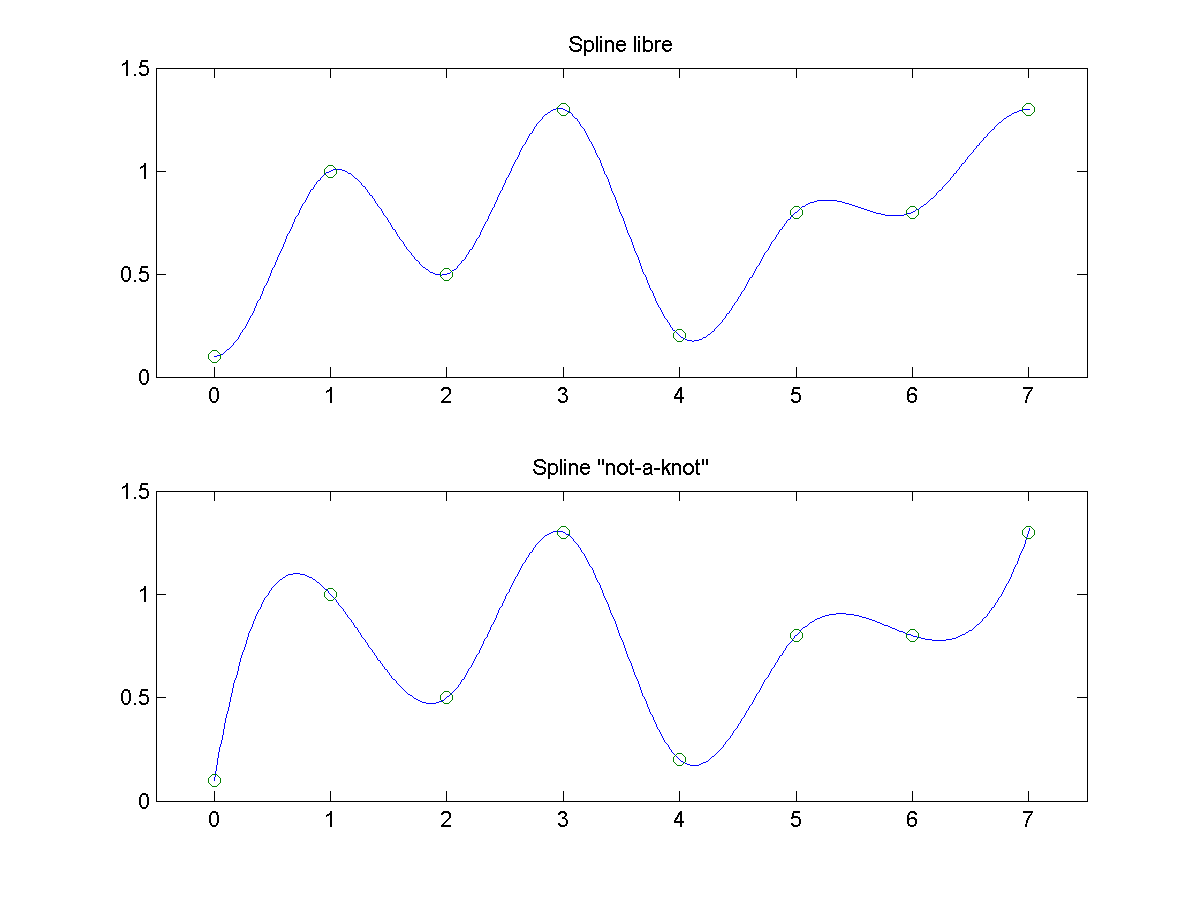
\includegraphics[scale=0.55]{images/spline-cubique}
    \end{center}
    \caption{Interpolation by cubic splines}
              \label{fig-spline-cubic}
\end{figure}
\end{exo}
